\subsection{The Hausdorff completion of a semi-local ring}

PROPOSITION 17. Let A be a commutative ring and \((\mathfrak{m}_{\lambda})_{\lambda \in L}\) a family of ideals of A, distinct from A, such that \(\mathfrak{m}_{\lambda}\) and \(\mathfrak{m}_{\mu}\) are relatively prime for \(\lambda \neq \mu\) . For every family \(s = (s(\lambda))_{\lambda \in L}\) of integers \(\geqslant 0\) , of finite support, set \(\mathfrak{a}_{s} = \bigcap_{\lambda \in L} \mathfrak{m}_{\lambda}^{s(\lambda)}\) (equal to the product of the \(\mathfrak{m}_{\lambda}^{s(\lambda)}\) for the \(\lambda\) such that \(s(\lambda) \neq 0\) ; cf.~Chapter II, § 1, no. 2, Propositions 3 and 5); the \(\mathfrak{a}_{s}\) form a fundamental system of neighbourhoods of 0 with respect to a topology \(\mathcal{T}\) compatible with the ring structure on A; let \(\hat{\mathbf{A}}\) be the Hausdorff completion of A with respect to this topology. On the other hand, for all \(\lambda \in L\) , let \(\mathbf{A}_{\lambda}\) be the ring A with the \(\mathfrak{m}_{\lambda}\) -adic topology and let \(\hat{\mathbf{A}}_{\lambda}\) be its Hausdorff completion. If \(u: \mathbf{A} \to \prod_{\lambda \in L} \mathbf{A}_{\lambda}\) denotes the diagonal homomorphism, \(u\) is continuous and the corresponding homomorphism \(\hat{u}\) :

\[
\hat {\mathbf {A}} \rightarrow \left(\prod_ {\lambda \in \mathbf {L}} \mathbf {A} _ {\lambda}\right) ^ {\wedge} = \prod_ {\lambda \in \mathbf {L}} \hat {\mathbf {A}} _ {\lambda}
\]

(General Topology, Chapter III, § 6, no. 5 and Chapter II, § 3, no. 9, Corollary 2 to Proposition 18) is a topological ring isomorphism.

The first assertion follows from General Topology, Chapter III, § 6, no. 3, Example 3. Let us set \(\mathbf{B} = \prod_{\lambda \in \mathbf{L}} \mathbf{A}_{\lambda}\) ; as the topology on \(\mathbf{A}\) is finer than each of the \(m_{\lambda}\) -adic topologies, the mappings \(\mathrm{pr}_{\lambda} \circ u\) are continuous and hence \(u\) is continuous. Also, \(u(a_s)\) is the intersection of the diagonal \(\Delta\) of \(\mathbf{B}\) and the open set \(\bigcap_{\lambda \in \mathbf{L}} \mathrm{pr}_{\lambda}^{-1}(m_{\lambda}^{s(\lambda)})\) of \(\mathbf{B}\) ; it follows that \(u\) is a strict morphism from the additive group \(\mathbf{A}\) to \(\mathbf{B}\) with image \(\Delta\) . Now \(\Delta\) is dense in \(\mathbf{B}\) . For let \(b = (a_{\lambda})_{\lambda \in \mathbf{L}}\) be an element of \(\mathbf{B}\) ; every neighbourhood of \(b\) in \(\mathbf{B}\) contains a set of the form \(b + \mathbf{V}\) , where \(\mathbf{V} = \bigcap_{\lambda \in \mathbf{L}} \mathrm{pr}_{\lambda}^{-1}(m_{\lambda}^{s(\lambda)})\) for a family \(s = (s(\lambda))_{\lambda \in \mathbf{L}}\) with finite support of integers \(\geqslant 0\) . As the \(m_{\lambda}^{s(\lambda)}\) are relatively prime in pairs (Chapter II, § 1, no. 2, Proposition 3), there exists \(x \in \mathbf{A}\) such that \(x \equiv a_{\lambda}\) (mod. \(m_{\lambda}^{s(\lambda)}\) ) for all \(\lambda\) (loc. cit., Proposition 5) and hence \((b + \mathbf{V}) \cap \Delta \neq \varnothing\) . The Hausdorff completion of the group \(\mathbf{B}/\Delta\) is then \(\{0\}\) ; applying Lemma 2 of no. 12 to the exact sequences \(0 \to \mathbf{A} \xrightarrow{u} \mathbf{B}, \mathbf{A} \xrightarrow{u} \mathbf{B} \to \mathbf{B}/\Delta\) , we see that \(\hat{u}\) is an isomorphism of \(\hat{\mathbf{A}}\) onto \(\hat{\mathbf{B}}\) .

COROLLARY. Let A be a principal ideal domain and P a representative system of extremal elements of A (Algebra, Chapter VII, § 1, no. 3). The topology on A with respect to which the ideals \(\neq0\) of A form a fundamental system of neighbourhoods of 0, which is compatible with the ring structure on A, is Hausdorff and the completion of A with this topology is canonically isomorphic to the product of the completions of A with respect to the \(\pi\) -adic topologies, where \(\pi\) runs through P.

The principal ideals \((\pi)\) where \(\pi \in P\) are maximal and distinct and hence relatively prime, we have already seen (no. 12, Example 3) that the \(\pi\) -adic topologies are Hausdorff and hence so is the topology defined in the statement of Proposition 17, which is finer than each of the \(\pi\) -adic topologies.

If the Corollary to Proposition 17 is applied when A = Z, we denote by \(\hat{Z}\) the completion of Z with respect to the topology for which all the ideals \(\neq0\) of Z form a fundamental system of neighbourhoods of 0, the ring isomorphic to the product \(\prod_{p\in P}Z_{p}\) of the rings of p-adic integers (P being the set of prime numbers).

\textbf{Remarks}\par

\begin{enumerate}
\def\labelenumi{(\arabic{enumi})}
\item
  Clearly, under the conditions of Proposition 17, the topology \(\mathcal{T}\) is the least upper bound of the \(m_{\lambda}\) -adic topologies on \(\mathbf{A}\) .
\item
  Every closed ideal \(\mathfrak{a}\) of \(\prod_{\lambda \in L} \hat{\mathbf{A}}_{\lambda}\) is identical with the product of its projections \(\mathfrak{a}_{\lambda} = \operatorname{pr}_{\lambda}(\mathfrak{a})\) , which are closed ideals in the \(\hat{\mathbf{A}}_{\lambda}\) ; for \(\hat{\mathbf{A}}_{\lambda}\) is canonically identified with a closed ideal \(\mathbf{A}_{\lambda}'\) of \(\prod_{\lambda} \hat{\mathbf{A}}_{\lambda}\) and \(\mathfrak{a}_{\lambda}\) with \(\mathfrak{a} \cap \mathbf{A}_{\lambda}'\) (Algebra, Chapter I, § 8, no. 10, Proposition 6), the sum of the \(\mathfrak{a}_{\lambda}\) is dense in the product \(\prod_{\lambda} \mathfrak{a}_{\lambda}\) (General Topology, Chapter III, § 2, no. 9, Proposition 25) and the latter is closed in \(\prod_{\lambda} \hat{\mathbf{A}}_{\lambda}\) , whence our assertion.
\end{enumerate}

PROPOSITION 18. Let A be a commutative ring, \((\mathfrak{m}_i)_{1 \leqslant i \leqslant q}\) a finite family of distinct maximal ideals of A, r the product ideal \(\mathfrak{m}_1\mathfrak{m}_2 \ldots \mathfrak{m}_q = \mathfrak{m}_1 \cap \mathfrak{m}_2 \cap \cdots \cap \mathfrak{m}_q\) and S the multiplicative subset \(\bigcap_{i=1}^{q} (\mathbf{A} - \mathfrak{m}_i)\) . Let A be given the r-adic topology, the ring \(\mathbf{B} = \mathbf{S}^{-1}\mathbf{A}\) the rB-adic topology and each of the local rings \(\mathbf{A}_{\mathfrak{m}_i}\) the \((\mathfrak{m}_i\mathbf{A}_{\mathfrak{m}_i})\) -adic topology. Let \(u: \mathbf{A} \to \mathbf{B}\) , \(v_i: \mathbf{B} \to \mathbf{A}_{\mathfrak{m}_i}\) be the canonical homomorphisms (Chapter II, § 2, no.1, Corollary 2 to Proposition 2) and \(v\) the homomorphism \((v_i): \mathbf{B} \to \prod_{i=1}^{q} \mathbf{A}_{\mathfrak{m}_i}\) . The homomorphisms \(u\) and \(v\) are continuous and the corresponding homomorphisms \(\hat{u}: \hat{\mathbf{A}} \to \hat{\mathbf{B}}\) and \(\hat{v}: \hat{\mathbf{B}} \to \prod_{i=1}^{q} (\mathbf{A}_{\mathfrak{m}_i})^{\wedge}\) are topological ring isomorphisms.

\(m_{i} \cap S = \varnothing\) for \(1 \leqslant i \leqslant q\) , hence the ideal \(m_{i}' = m_{i}B\) of B is maximal (Chapter II, §2, no. 5, Proposition 11) and

\[
\mathfrak {r B} = \mathfrak {m} _ {1} ^ {\prime} \cap \mathfrak {m} _ {2} ^ {\prime} \cap \dots \cap \mathfrak {m} _ {q} ^ {\prime}
\]

(Chapter II, §2, no. 4); finally, \(\mathbf{B}_{\mathfrak{m}_i'} = \mathbf{A}_{\mathfrak{m}_i}\) up to a canonical isomorphism (Chapter II, §2, no. 5, Proposition 11). As \(\bar{u}^{-1}(\mathfrak{rB}) = \mathfrak{r}\) and \(\bar{v}_i^{-1}(m_i\mathbf{A}_{\mathfrak{m}_i}) \supset \mathfrak{rB}\) , \(u\) and \(v\) are continuous. Then it is sufficient to prove that,

\[
w = v \circ u: \mathrm{A} \rightarrow \prod_ {i = 1} ^ {q} \mathrm{A} _ {\mathfrak {m} _ {i}},
\]

\(\hat{w}\) is an isomorphism of \(\hat{\mathbf{A}}\) onto \(\prod_{i=1}^{q} \hat{\mathbf{A}}_{m_i}\) , for this result applied to B and the \(m_i'\) will show that \(\hat{v}\) is an isomorphism and therefore also \(\hat{u}\) . Note that every product of powers of the \(m_i\) contains a power of r and hence the r-adic topology is the least upper bound of the \(m_i\) -adic topologies; moreover, if \(A_i\) denotes the

\[
\mathfrak {m} _ {i} \text {-adic}
\]

\[
\phi : \mathrm{A} \rightarrow \prod_ {i = 1} ^ {q} \mathrm{A} _ {i}
\]

\(\hat{\phi}:\hat{\mathbf{A}}\to \prod_{i = 1}^{q}\hat{\mathbf{A}}_i\) is an isomorphism (Proposition 17). Then it all amounts to proving that, if \(u_{i}:\mathbf{A}_{i}\rightarrow \mathbf{A}_{m_{i}}\) is the canonical mapping, \(\hat{u}_i\colon \hat{\mathbf{A}}_i\to \hat{\mathbf{A}}_{m_i}\) is an isomorphism. Now, for all \(n\) , the mapping

\[
u _ {i, n} \colon \mathrm{A} / \mathfrak {m} _ {i} ^ {n} \rightarrow \mathrm{A} _ {\mathfrak {m} _ {i}} / \mathfrak {m} _ {i} ^ {n} \mathrm{A} _ {\mathfrak {m} _ {i}}
\]

derived from \(u_{i}\) by taking quotients is an isomorphism (Chapter II, § 3, no. 3, Proposition 9); our assertion follows from the fact that \(\hat{\mathbf{A}}_i\) (resp. \(\hat{\mathbf{A}}_{\mathfrak{m}_i}\) ) is the inverse limit of the discrete rings \(\mathbf{A} / \mathfrak{m}_i^n\) (resp. \(\mathbf{A}_{\mathfrak{m}_i} / \mathfrak{m}_i^n \mathbf{A}_{\mathfrak{m}_i}\) ) (cf.~no. 6).

Remark (3). We see that an integral domain A can be such that its Hausdorff completion \(\hat{A}\) admits non-zero divisors of zero.

PROPOSITION 19. Let A be a commutative ring and m a maximal ideal of A. The Hausdorff completion \(\hat{\mathbf{A}}\) of A with respect to the m-adic topology is a local ring whose maximal ideal is \(\hat{\mathfrak{m}}\) .

If \(\mathfrak{a} = \bigcap_{k\geqslant 1}\mathfrak{m}^k\) , \(\hat{\mathbf{A}}\) is the completion of the Hausdorff ring \(\mathbf{A} / \mathfrak{a}\) associated with \(\mathbf{A}\) and, as \(\mathfrak{m} / \mathfrak{a}\) is maximal in \(\mathbf{A} / \mathfrak{a}\) , we may assume that \(\mathbf{A}\) is Hausdorff with respect to the \(\mathfrak{m}\) -adic topology. As \(\mathbf{A} / \mathfrak{m}\) and \(\hat{\mathbf{A}} /\hat{\mathfrak{m}}\) are isomorphic rings (no. 12, formula (21)), \(\hat{\mathfrak{m}}\) is maximal in \(\hat{\mathbf{A}}\) . As the topology on \(\hat{\mathbf{A}}\) is defined by the filtration \((\mathfrak{m}^n)^{\wedge}\) (no. 12), the proposition will be a consequence of the following lemma:

LEMMA 3. Let A be a complete Hausdorff topological ring, in which there exists a fundamental system \(\mathfrak{S}\) of neighbourhoods of 0 consisting of additive subgroups of A.

\begin{enumerate}
\def\labelenumi{(\roman{enumi})}
\item
  For all \(x \in \mathbf{A}\) such that \(\lim_{n \to \infty} x^n = 0\) , \(1 - x\) is invertible in \(\mathbf{A}\) and its inverse is equal to \(\sum_{n=0}^{\infty} x^n\) .
\item
  Let \(\mathfrak{a}\) be a two-sided ideal of A such that \(\lim x^n = 0\) for all \(x \in \mathfrak{a}\) . For an element y of A to be invertible, it is necessary and sufficient that its class mod. a be invertible in A/a; in particular a is contained in the Jacobson radical of A.
\end{enumerate}

(i) As

\[
(1 - x) (1 + x + \dots + x ^ {n}) = (1 + x + \dots + x ^ {n}) (1 - x) = 1 - x ^ {n + 1},
\]

it all amounts to proving that the series with general term \(x^{n}\) is convergent in A; now, by hypothesis, for every neighbourhood \(V \in \mathfrak{S}\) of 0 in A, there exists an integer p \textgreater{} 0 such that \(x^{n} \in V\) for all \(n \geqslant p\) . We conclude that

\[
x ^ {p} + x ^ {p + 1} + \dots + x ^ {q} \in \mathbf {V}
\]

for all \(q \geqslant p\) and our assertion then follows from Cauchy's criterion (General Topology, Chapter III, § 5, no. 2, Theorem 1).

\begin{enumerate}
\def\labelenumi{(\roman{enumi})}
\setcounter{enumi}{1}
\tightlist
\item
  Suppose that there exists \(y' \in A\) such that \(yy' \equiv 1 \pmod{a}\) and \(y'y \equiv 1 \pmod{a}\) . The hypothesis on \(a\) implies, by (i), that \(yy'\) and \(y'y\) are invertible in \(A\) and hence \(y\) is invertible in \(A\) . In particular, every \(x \in a\) is such that \(1 - x\) is invertible in \(A\) and, as \(a\) is a two-sided ideal of \(A\) , it is contained in the Jacobson radical of \(A\) (Algebra, Chapter VIII, § 6, no. 3, Theorem 1).
\end{enumerate}

Having established this lemma, it is sufficient to apply it to the topological ring \(\hat{\mathbf{A}}\) and the ideal \(\hat{\mathfrak{m}}\) , as, for all \(x \in \hat{\mathfrak{m}}\) , \(x^n \in (\hat{\mathfrak{m}})^n \subset (\mathfrak{m}^n)^\wedge\) and the sequence \((x^n)\) therefore tends to 0.

If we take A = Z, every maximal ideal of Z is of the form pZ where p is prime. The ring of p-adic numbers \(Z_{p}\) is then a local ring of which \(pZ_{p}\) is the maximal ideal (Corollary 2 to Proposition 16) and whose residue field is isomorphic to \(Z/pZ = F_{p}\) , and \(\mathbf{Z}_{(p)}\) with the \(pZ_{(p)}\) -adic topology is identified with a topological subring of \(Z_{p}\) containing Z.

COROLLARY. Let A be a semi-local ring (Chapter II, § 3, no. 5), \(\mathfrak{m}_i\) its distinct maximal ideals ( \(1 \leqslant i \leqslant q\) ) and

\[
\mathfrak {r} = \mathfrak {m} _ {1} \cap \mathfrak {m} _ {2} \cap \dots \cap \mathfrak {m} _ {q}
\]

its Jacobson radical. The Hausdorff completion \(\hat{\mathbf{A}}\) of \(\mathbf{A}\) with respect to the \(\mathfrak{r}\) -adic topology is a semi-local ring, canonically isomorphic to the product \(\prod_{i=1}^{q} \hat{\mathbf{A}}_{\mathfrak{m}_i}\) , where \(\hat{\mathbf{A}}_{\mathfrak{m}_i}\) is the Hausdorff completion ring of the local ring \(\mathbf{A}_{\mathfrak{m}_i}\) with respect to the \((\mathfrak{m}_i\mathbf{A}_{\mathfrak{m}_i})\) -adic topology.

\section{m-ADIC TOPOLOGIES ON NOETHERIAN RINGS}

All the filtrations considered in this paragraph are assumed to be exhaustive.

\subsection{Good filtrations}

Let A be a filtered commutative ring, E a filtered A-module and \((A_{n})\) and \((E_{n})\)

the respective filtrations of A and E; suppose that \(A_{0} = A\) . In the polynomial ring A{[}X{]} the set \(A' = \sum_{n \geqslant 0} A_{n} X^{n}\) is a graded sub-A-algebra of type N; the subgroup \(E' = \sum_{n \geqslant 0} E_{n} \otimes_{A} A X^{n}\) of \(E \otimes_{A} A[X]\) is a graded \(A'\) -module of type N, since

\[
\mathbf {A} _ {m} \mathbf {X} ^ {m} (\mathrm{E} _ {n} \otimes_ {\mathbf {A}} \mathbf {A X} ^ {n}) \subset (\mathbf {A} _ {m} \mathrm{E} _ {n} \otimes_ {\mathbf {A}} \mathbf {A X} ^ {m + n}) \subset \mathrm{E} _ {m + n} \otimes_ {\mathbf {A}} \mathbf {A X} ^ {m + n}.
\]

DEFINITION 1. Let A be a commutative ring, m an ideal of A, E an A-module and \((\mathrm{E}_{n})\) a filtration on the additive group E consisting of submodules of E. The filtrations \((\mathrm{E}_{n})\) is called m-good if:

\begin{enumerate}
\def\labelenumi{(\arabic{enumi})}
\item
  \(\mathfrak{m}\mathrm{E}_n\subset \mathrm{E}_{n + 1}\) for all \(n\in \mathbf{Z}\) ;
\item
  there exists an integer \(n_0\) such that \(\mathfrak{m}\mathrm{E}_n = \mathrm{E}_{n+1}\) for \(n \geqslant n_0\) .
\end{enumerate}

Then by induction on \(q\) , \(\mathfrak{m}^q\mathrm{E}_n = \mathrm{E}_{n + q}\) for \(n \geqslant n_0\) , \(q \geqslant 1\) . Note that condition (1) means that the filtration \((\mathrm{E}_n)\) is compatible with the A-module structure on E if A is given the m-adic filtration. Clearly, on every A-module E, the m-adic filtration is m-good. If a filtration on an A-module E is m-good, the quotient filtration on any quotient module of E is m-good.

THEOREM 1. Let A be a commutative ring, m an ideal of A, E an A-module and \((\mathrm{E}_{n})\) a filtration of the additive group E consisting of finitely generated sub-A-modules. Suppose that \(mE_{n} \subset E_{n+1}\) for all n.~Let \(A'\) be the graded subalgebra \(\sum_{n \geqslant 0} m^{n} X^{n}\) of A{[}X{]} and \(E'\) the graded \(A'\) -module \(\sum_{n \geqslant 0} E_{n} \otimes_{A} AX^{n}\) . The two following conditions are equivalent:

\begin{enumerate}
\def\labelenumi{(\alph{enumi})}
\item
  The filtration \((\mathbf{E}_n)\) is m-good.
\item
  E' is a finitely generated A'-module.
\end{enumerate}

Suppose that \(mE_{n-1} = E_n\) for \(n > n_0 \geqslant 0\) . For \(i \leqslant n_0\) , let \((e_{ij})_{1 \leqslant j \leqslant r_i}\) be a finite system of generators of the A-module \(E_i\) . As the A-module \(E_n \otimes_A X^n\) is generated by the elements \(e_{nj} \otimes X^n\) for \(0 \leqslant n \leqslant n_0\) and is equal to

\[
\mathfrak {m} ^ {n - n _ {0}} \mathrm{E} _ {n _ {0}} \otimes_ {\mathbf {A}} \mathrm{AX} ^ {n}
\]

for \(n > n_0\) , the A'-module E' is generated by the elements \(e_{nj} \otimes \mathbf{X}^n\) for \(0 \leqslant n \leqslant n_0\) and \(1 \leqslant j \leqslant r_n\) ; then it is certainly finitely generated.

Conversely, if \(\mathbf{E}'\) is a finitely generated \(\mathbf{A}'\) -module, it is generated by a finite family of elements of the form \(e_k \otimes \mathbf{X}^{n(k)}\) , where \(e_k \in \mathbf{E}_{n(k)}\) . Let \(n_0\) be the greatest of the integers \(n(k)\) . Then for \(n \geqslant n_0\) and \(f \in \mathbf{E}_n\) ,

\[
f \otimes \mathbf {X} ^ {n} = \sum_ {k} t _ {k} (e _ {k} \otimes \mathbf {X} ^ {n (k)})
\]

where \(t_k \in \mathbf{A}'\) ; replacing if need be \(t_k\) by its homogeneous component of degree \(n - n(k)\) , we may assume that \(t_k = a_k \mathbf{X}^{n - n(k)}\) , where \(a_k \in \mathfrak{m}^{n - n(k)}\) .

As the unique element \(X^{n}\) forms a basis of the A-module \(AX^{n}\) , the equation \(f \otimes X^{n} = \left( \sum_{k} a_{k} e_{k} \right) \otimes X^{n}\) implies \(f = \sum_{k} a_{k} e_{k}\) . Then \(E_{n} \subset m^{n-n_{0}} E_{n_{0}}\) ; since the opposite inclusion is obvious,

\[
\mathrm{E} _ {n} = \mathfrak {m} ^ {n - n _ {0}} \mathrm{E} _ {n _ {0}},
\]

whence \(\mathbf{E}_n = m\mathbf{E}_{n - 1}\) for \(n > n_0\)

LEMMA 1. Let A be a commutative Noetherian ring and m an ideal of A. Then the subring \(\mathbf{A}' = \sum_{n\geqslant 0}\mathfrak{m}^n\mathbf{X}^n\) of A{[}X{]} is Noetherian.

A' is an A-algebra generated by mX; as A is Noetherian, mX is a finitely generated A-module and the conclusion then follows from § 2, no. 10, Corollary 3 to Theorem 2.

PROPOSITION 1. Let A be a commutative Noetherian ring and m an ideal of A; let A be given the m-adic filtration. Let E, F be two filtered A-modules and j: F → E an injective homomorphism compatible with the filtrations. If E is finitely generated and its filtration is m-good, then F is finitely generated and its filtration is m-good.

As F is isomorphic to a submodule of E, it is finitely generated since A is Noetherian and E is finitely generated. Let \((\mathbf{E}_{n})\) , \((\mathbf{F}_{n})\) be the respective filtrations on E and F, which consist of finitely generated submodules; preserving the notation of Lemma 1, we set \(E' = \sum_{n \geqslant 0} E_{n} \otimes_{A} AX^{n}\) , \(F' = \sum_{n \geqslant 0} F_{n} \otimes_{A} AX^{n}\) ; as by hypothesis \(F_{n}\) is isomorphic to a submodule of \(E_{n}\) , we see that \(F'\) is isomorphic to a submodule of \(E'\) . By Theorem 1, \(E'\) is a finitely generated \(A'\) -module and hence so is \(F'\) since \(A'\) is Noetherian (Lemma 1). Hence the conclusion by virtue of Theorem 1.

COROLLARY 1 (the Artin-Rees Lemma). Let A be a commutative Noetherian ring, m an ideal of A, E a finitely generated A-module and F a submodule of E. The filtration induced on F by the m-adic filtration on E is m-good.

In other words, there exists an integer \(n_{0}\) such that

\[
\mathfrak {m} ((\mathfrak {m} ^ {n} \mathrm{E}) \cap \mathrm{F}) = (\mathfrak {m} ^ {n + 1} \mathrm{E}) \cap \mathrm{F}\tag{1}
\]

for all \(n \geqslant n_0\) .

COROLLARY 2. Let A be a commutative Noetherian ring and a, b two ideals of A. There exists an integer h \textgreater{} 0 such that \(a^{h} \cap b \subset ab\) .

There exists \(n\) such that \(\mathfrak{a}^{n+1} \cap \mathfrak{b} = \mathfrak{a}(\mathfrak{a}^n \cap \mathfrak{b}) \subset \mathfrak{ab}\) by Corollary 1 applied to \(\mathbf{E} = \mathbf{A}, \mathbf{F} = \mathfrak{b}\) .

COROLLARY 3. Let A be a commutative Noetherian ring, m an ideal of A and x an element of A which is not a divisor of 0. There exists an integer \(k > 0\) such that, for all \(n \geqslant k\) , the relation \(xy \in \mathfrak{m}^n\) implies \(y \in \mathfrak{m}^{n - k}\) .

Corollary 1 applied to \(\mathbf{E} = \mathbf{A}\) , \(\mathbf{F} = \mathbf{A}x\) shows that there exists \(k\) such that, for all \(n \geqslant k\) , \(\mathfrak{m}^n \cap \mathbf{A}x = \mathfrak{m}^{n - k}(\mathfrak{m}^k \cap \mathbf{A}x)\) . Then, if \(xy \in \mathfrak{m}^n\) ,

\[
x y \in \mathfrak {m} ^ {n} \cap A x \subset \mathfrak {m} ^ {n - k} x
\]

and, as \(x\) is not a divisor of 0, we deduce that \(y \in \mathfrak{m}^{n - k}\) .

In the notation of transporters (Chapter I, § 2, no. 10), the conclusion of Corollary 3 reads

\[
\mathfrak {m} ^ {n}: \mathrm{A} x \subset \mathfrak {m} ^ {n - k}.\tag{2}
\]

COROLLARY 4. Let A be a commutative Noetherian ring, m an ideal of A, E a finitely generated A-module and \((\mathbf{E}_{n})\) and \((\mathbf{E}_{n}^{\prime})\) two filtrations consisting of submodules of E. Suppose that the filtrations \((\mathbf{E}_{n})\) and \((\mathbf{E}_{n}^{\prime})\) are compatible with the A-module structure on E when A is given the m-adic filtration. If the filtration \((\mathbf{E}_{n})\) is m-good and \(E_{n}^{\prime} \subset E_{n}\) for all \(n \in Z\) , the filtration \((\mathbf{E}_{n}^{\prime})\) is m-good. This a special case of Proposition 1.

LEMMA 2. Let A, B be two commutative Noetherian rings, \(\phi: \mathrm{A} \to \mathrm{B}\) a ring homomorphism, E a finitely generated A-module and F a finitely generated B-module. Then \(\operatorname{Hom}_{\mathbf{A}}(\mathrm{E}, \phi_*(\mathrm{F}))\) is a finitely generated B-module.

There exists by hypothesis a surjective A-homomorphism \(v: \mathbf{A}^n \to \mathbf{E}\) ; the mapping \(u \mapsto u \circ v\) of \(\operatorname{Hom}_{\mathbf{A}}(\mathbf{E}, \phi_*(\mathbf{F}))\) to \(\operatorname{Hom}_{\mathbf{A}}(\mathbf{A}^n, \phi_*(\mathbf{F}))\) is therefore injective and, as B is Noetherian, it is sufficient to prove that \(\operatorname{Hom}_{\mathbf{A}}(\mathbf{A}^n, \phi_*(\mathbf{F}))\) is a finitely generated B-module; which is immediate since it is isomorphic to \(\mathbf{F}^n\) .

PROPOSITION 2. Let A be a commutative Noetherian ring, m an ideal of A and E, F two finitely generated A-modules. If \((\mathbf{F}_{n})\) is an m-good filtration on F, the submodules \(\operatorname{Hom}_{\mathbf{A}}(\mathbf{E}, \mathbf{F}_{n})\) form an m-good filtration on the A-module \(\operatorname{Hom}_{\mathbf{A}}(\mathbf{E}, \mathbf{F})\) . As \(m^{k}F_{n}\subset F_{n+k}\) for \(n\in Z, k\geqslant0\) , it is also true that

\[
\mathfrak {m} ^ {k} \operatorname{Hom} _ {\mathbf {A}} (\mathrm{E}, \mathrm{F} _ {n}) \subset \operatorname{Hom} _ {\mathbf {A}} (\mathrm{E}, \mathrm{F} _ {n + k});
\]

the family \((\mathrm{Hom}_{\mathbf{A}}(\mathrm{E},\mathrm{F}_{n}))_{n\in\mathbf{Z}}\) is then a filtration on \(\mathrm{Hom}_{\mathbf{A}}(\mathrm{E},\mathbf{F})\) compatible with its module structure over the ring A filtered by the m-adic filtration. Since E is finitely generated, there exists an integer r\textgreater0 and a surjective A-homomorphism \(u:A^{r}\rightarrow E\) which defines an injective A-homomorphism

\[
v = \operatorname{Hom} (u, 1 _ {\mathrm{F}}): \operatorname{Hom} _ {\mathrm{A}} (\mathrm{E}, \mathrm{F}) \rightarrow \operatorname{Hom} _ {\mathrm{A}} (\mathrm{A} ^ {r}, \mathrm{F});
\]

clearly \(v\) is compatible with the filtrations \((\mathrm{Hom}_{\mathbf{A}}(\mathbf{E},\mathbf{F}_n))\) and \((\mathrm{Hom}_{\mathbf{A}}(\mathbf{A}^r,\mathbf{F}_n))\) . As \(\mathrm{Hom}_{\mathbf{A}}(\mathbf{E},\mathbf{F})\) and \(\mathrm{Hom}_{\mathbf{A}}(\mathbf{A}^r,\mathbf{F})\) are finitely generated (Lemma 2), it is sufficient by virtue of Proposition 1 to show that the filtration \((\mathrm{Hom}_{\mathbf{A}}(\mathbf{A}^{r},\mathbf{F}_{n}))\) is m-good; but this is immediate by virtue of the existence of the canonical isomorphism \(\mathrm{Hom}_{\mathbf{A}}(\mathbf{A}^{r},\mathbf{F}_{n})\to \mathbf{F}_{n}^{r}\) and the fact that the relation \(\mathfrak{mF}_n = \mathbf{F}_{n + 1}\) implies \(\mathfrak{m}(\mathbf{F}_n^r) = (\mathfrak{m}\mathbf{F}_n)^r = \mathbf{F}_{n + 1}^r\) (Algebra, Chapter II, § 3, no. 7, Remark).

PROPOSITION 3. Let A be a Noetherian ring and m an ideal of A such that A is Hausdorff and complete with respect to the m-adic topology. Let E be a filtered A-module over the filtered ring A, the filtration ( \(E_{n}\) ) of E being such that \(E_{0} = E\) and E is Hausdorff with respect to the topology defined by ( \(E_{n}\) ). Then the following conditions are equivalent:

\begin{enumerate}
\def\labelenumi{(\alph{enumi})}
\item
  E is a finitely generated A-module and \((\mathbf{E}_{n})\) is an m-good filtration.
\item
  gr(E) is a finitely generated gr(A)-module.
\item
  For all \(n \geqslant 0\) , \(\mathrm{gr}_n(\mathbf{E})\) is a finitely generated A-module and there exists \(n_0\) such that for \(n \geqslant n_0\) the canonical homomorphism

\[
\operatorname{gr} _ {1} (\mathrm{A}) \otimes_ {\mathrm{A}} \operatorname{gr} _ {n} (\mathrm{E}) \rightarrow \operatorname{gr} _ {n + 1} (\mathrm{E})\tag{3}
\]

is surjective.
\end{enumerate}

It follows immediately from the definitions that (a) implies (c). The fact that (b) implies (c) is a consequence of § 1, no. 3, Lemma 1; conversely, if (c) holds, clearly gr(E) is generated as a gr(A)-module by the sum of the gr \(_{p}\) (E) for p ≤ n \(_{0}\) and hence by hypothesis admits a finite system of generators. It remains to prove that (c) implies (a); as the gr \(_{n}\) (E) are finitely generated and E \(_{0}\) = E, clearly first, by induction on n, E/E \(_{n}\) is a finitely generated A-module for all n; it will therefore be sufficient to prove that, for n \textgreater{} n \(_{0}\) , E \(_{n}\) is a finitely generated A-module and that mE \(_{n}\) = E \(_{n+1}\) . Now, consider the A-module E \(_{n+1}\) with the exhaustive and separated filtration (E \(_{n+k}\) )(k ≥ 1); mE \(_{n}\) ⊂ E \(_{n+1}\) ; hypothesis (c) implies that the image of mE \(_{n}\) in gr \(_{n+1}\) (E) = E \(_{n+1}\) /E \(_{n+2}\) is equal to gr \(_{n+1}\) (E) and generates the graded gr(A)-module gr(E \(_{n+1}\) ). As gr \(_{n+1}\) (E) is by hypothesis a finitely generated A-module, it follows from § 2, no. 9, Proposition 12 that mE \(_{n}\) = E \(_{n+1}\) and that E \(_{n+1}\) is a finitely generated A-module.

\subsection{m-adic topologies on Noetherian rings}

PROPOSITION 4. Let A be a commutative Noetherian ring, m an ideal of A and E a finitely generated A-module. All the m-good filtrations on E define the same topology (namely the m-adic topology).

Let \((\mathbf{E}_{n})\) be an m-good filtration on E. As this filtration is exhaustive, every element of E belongs to one of the \(E_{n}\) and, as E is finitely generated and the \(E_{n}\) are A-modules, there exists an integer \(n_{1}\) such that \(E_{n_{1}} = E\) . On the other hand let \(n_{0}\) be such that \(mE_{n} = E_{n+1}\) for \(n \geqslant n_{0}\) ; then, for \(n > n_{0} - n_{1}\) , \(m^{n}E \subset E_{n+n_{1}} = m^{n+n_{1}-n_{0}}E_{n_{0}} \subset m^{n+n_{1}-n_{0}}E\) , which proves the proposition.

THEOREM 2 (Krull). Let A be a commutative Noetherian ring, m an ideal of A, E a finitely generated A-module and F a submodule of E. Then the m-adic topology on F is induced by the m-adic topology on E.

It follows from no. 1, Proposition 1 that the filtration induced on F by the m-adic filtration on E is m-good and the conclusion then follows from Proposition 4.

COROLLARY. Let A be a commutative Noetherian ring, m an ideal of A, E an A-module and F a finitely generated A-module. Every A-linear mapping u: E → F is a strict morphism (General Topology, Chapter III, § 2, no. 8) for the m-adic topologies.

As \(u(\mathfrak{m}^{n}\mathbf{E}) = \mathfrak{m}^{n}u(\mathbf{E})\) , u is a strict morphism of E onto \(u(\mathbf{E})\) for the m-adic topologies on these two modules and the m-adic topology on \(u(\mathbf{E})\) is induced by the m-adic topology on F by Theorem 2.

PROPOSITION 5. Let A be a commutative Noetherian ring, m an ideal of A and E a finitely generated A-module. The closure \(\bigcap_{n=1}^{\infty} \mathfrak{m}^{n}\mathrm{E}\) of \(\{0\}\) in E with respect to the m-adic topology is the set of \(x \in \mathrm{E}\) for which there exists an element \(m \in \mathfrak{m}\) such that \((1 - m)x = 0\) . If \(x = mx\) where \(m \in \mathfrak{m}\) , \(x = m^{n}x \in \mathfrak{m}^{n}\mathrm{E}\) for every integer \(n \geqslant 0\) and hence \(x \in \mathrm{F} = \bigcap_{n=0}^{\infty} \mathfrak{m}^{n}\mathrm{E}\) . Conversely, if \(x \in \mathrm{F}\) , Ax is contained in the intersection of the neighbourhoods of 0 in E; it then follows from Theorem 2 that the m-adic topology on Ax, which is induced by that on E, is the coarsest topology; as mx is by definition a neighbourhood of 0 with this topology, mx = Ax and hence there exists \(m \in \mathfrak{m}\) such that \(x = mx\) .

We may also say that mF = F since

\[
\mathrm{F} = \bigcap_ {n = 1} ^ {\infty} m ^ {n + 1} \mathrm{E} \subset m. \bigcap_ {n = 1} ^ {\infty} m ^ {n} \mathrm{E} = m \mathrm{F};
\]

as A is Noetherian, F is a finitely generated A-module; it is then sufficient to apply Chapter II, § 2, no. 2, Corollary 3 to Proposition 4.

COROLLARY (Krull). Let A be a commutative Noetherian ring and m an ideal of A. The ideal \(\bigcap_{n=1}^{\infty}m^{n}\) is the set of elements \(x\in A\) for which there exists \(m\in m\) such that \((1-m)x=0\) . In particular, for \(\bigcap_{n=1}^{\infty}m^{n}=\{0\}\) , it is necessary and sufficient that no element of \(1+m\) be a divisor of 0 in A.

It is sufficient to apply Proposition 5 to \(\mathbf{E} = \mathbf{A}_s\) .

\pandocbounded{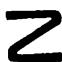
\includegraphics[keepaspectratio]{images/part002_69a966b6.jpg}}

Remark. The hypothesis that A is Noetherian is essential in this corollary. For example, let A be the ring of infinitely differentiable mappings from R to itself and let m be the (maximal) ideal of A consisting of the functions f such that \(f(0) = 0\) . It is immediate that \(\bigcap_{n=0}^{\infty} m^{n}\) is the set of functions f such that

\(f^{(n)}(0) = 0\) for all \(n \geqslant 0\) and there exist such functions with \(f(x) \neq 0\) , for all \(x \neq 0\) , for example the function \(f\) defined by \(f(x) = e^{-1 / x^2}\) for \(x \neq 0\) and \(f(0) = 0\) .

DEFINITION 1. Let A be a topological ring. If a two-sided ideal m of A is such that the given topology on A is the m-adic topology, m is called a defining ideal of the topology on A.

Let A be a commutative Noetherian ring, m an ideal of A and t its radical (Chapter II, § 2, no. 6). If \(m'\) is a defining ideal of the m-adic topology, there exists an integer n \textgreater{} 0 such that \(m'^{n} \subset m\) (§ 2, no. 5) and hence \(m' \subset t\) ; conversely, since A is Noetherian, there exists an integer k \textgreater{} 0 such that \(t^{k} \subset m\) (Chapter II, § 2, no. 6, Proposition 15) and hence t is the largest defining ideal of the m-adic topology.

\subsection{Zariski rings}

PROPOSITION 6. Let A be a commutative Noetherian ring and m an ideal of A. The following properties are equivalent:

\begin{enumerate}
\def\labelenumi{(\alph{enumi})}
\item
  \(\mathfrak{m}\) is contained in the Jacobson radical of A.
\item
  Every finitely generated A-module is Hausdorff with the m-adic topology.
\item
  For every finitely generated A-module E, every submodule of E is closed with respect to the m-adic topology on E.
\item
  Every maximal ideal of A is closed with respect to the m-adic topology.
\end{enumerate}

Let us show that (a) implies (b). Suppose that m is contained in the Jacobson radical of A and let E be a finitely generated A-module. If \(x \in E\) and \(m \in m\) are such that \((1 - m)x = 0\) , then x = 0, for 1 - m is invertible in A. Then (no. 2, Proposition 5) E is Hausdorff with the m-adic topology.

Let us prove that (b) implies (c). Suppose (b) holds. Let E be a finitely generated A-module and F a submodule of E. Then E/F is Hausdorff with the m-adic topology, which is the quotient topology of the m-adic topology on E; then F is closed in E.

Clearly (c) implies (d). Let us show finally that (d) implies (a). It follows from (d) that, for every maximal ideal a of A, the A-module A/a is Hausdorff with the m-adic topology. This implies \(\mathfrak{m}(\mathrm{A}/\mathfrak{a}) \neq \mathrm{A}/\mathfrak{a}\) , unless the m-adic topology on A/a were the coarsest topology and A/a were reduced to 0, which is absurd since A/a is a field. The canonical image of m in A/a is therefore an ideal of A/a distinct from A/a and hence reduced to 0; then \(m \subset a\) , which proves that m is contained in the Jacobson radical of A.

DEFINITION 2. A topological ring A is called a Zariski ring if it is commutative and Noetherian and there exists a defining ideal m for the topology on A satisfying the equivalent conditions of Proposition 6.

A Zariski ring A is necessarily Hausdorff (Proposition 6) and every defining ideal of its topology is contained in the Jacobson radical of A.

\textbf{Examples of Zariski rings}\par

\begin{enumerate}
\def\labelenumi{(\arabic{enumi})}
\item
  Let A be a commutative Noetherian ring and m an ideal of A. If A is Hausdorff and complete with the m-adic topology, A is a Zariski ring with this topology, by virtue of § 2, no. 13, Lemma 3.
\item
  Every quotient ring A/b of a Zariski ring is a Zariski ring, for it is Noetherian and, if m is a defining ideal of A, \(\mathfrak{m}(\mathbf{A}/\mathfrak{b}) = (\mathfrak{m} + \mathfrak{b})/\mathfrak{b}\) is contained in the Jacobson radical of A/b (Algebra, Chapter VIII, § 6, no. 3, Proposition 7).
\item
  Let A be a Noetherian semi-local ring and r its Jacobson radical. Then A with the r-adic topology is a Zariski ring. This will always be the topology in question (unless otherwise stated) when we consider a Noetherian semi-local ring as a topological ring.
\end{enumerate}

PROPOSITION 7. Let A, A' be two commutative rings and h: A → A' a ring homomorphism. Suppose that A is Noetherian and that A' is a finitely generated A-module (with the structure defined by h). Let m be an ideal of A and let m' = mA'. Then:

\begin{enumerate}
\def\labelenumi{(\roman{enumi})}
\item
  For the \(\mathfrak{m}'\) -adic topology on \(\mathbf{A}'\) to be Hausdorff, it is necessary and sufficient that the elements of \(1 + h(\mathfrak{m})\) be not divisors of 0 in \(\mathbf{A}'\) .
\item
  If A with the m-adic topology is a Zariski ring, then A' with the m'-adic topology is a Zariski ring.
\item
  If \(h\) is injective (thus identifying \(\mathbf{A}\) with a subring of \(\mathbf{A}'\) ), the \(\mathfrak{m}'\) -adic topology on \(\mathbf{A}'\) induces on \(\mathbf{A}\) the \(\mathfrak{m}\) -adic topology.
\end{enumerate}

Recall that the m'-adic filtration on A' coincides with the m-adic filtration on the A-module A' (§ 2, no. 1, Example 3). Assertion (i) is thus a special case of Proposition 5 of no. 2 and assertion (iii) a special case of Theorem 2 of no. 2, Finally let us show (ii). Suppose that A is a Zariski ring with the m-adic topology and let E' be a finitely generated A'-module; it is also a finitely generated A-module and the m-adic and m'-adic filtrations on E' coincide; then E' is Hausdorff with the m'-adic topology. Finally the A-module A' is Noetherian and hence the ring A' is Noetherian, which completes the proof that A' is a Zariski ring.

\subsection{The Hausdorff completion of a Noetherian ring}

Let A be a commutative ring, m an ideal of A and E an A-module; let \(\hat{A}\) and \(\hat{E}\) denote the respective Hausdorff completions of A and E with respect to the m-adic topology and \(j_{E}\) the canonical mapping \(E \rightarrow \hat{E}\) . The A-bilinear mapping \((a, x) \mapsto aj_{\mathrm{E}}(x)\) of \(\hat{A} \times E\) to \(\hat{E}\) defines an A-linear mapping

\[
\alpha_ {\mathrm{E}} \colon \hat {\mathrm{A}} \otimes_ {\mathrm{A}} \mathrm{E} \rightarrow \hat {\mathrm{E}},
\]

called canonical. Let \(u: \mathrm{E} \to \mathrm{F}\) be an A-module homomorphism and let \(\hat{u}\colon \hat{\mathbf{E}}\to \hat{\mathbf{F}}\) be the mapping obtained by passing to the Hausdorff completions; for \(a\in \hat{\mathbf{A}},x\in \mathbf{E},\)

\[
\alpha_ {\mathrm{F}} (a \otimes u (x)) = a j _ {\mathrm{F}} (u (x)) = a \hat {u} (j _ {\mathrm{E}} (x)) = \hat {u} (\alpha_ {\mathrm{E}} (a \otimes x)),
\]

in other words, the diagram

\pandocbounded{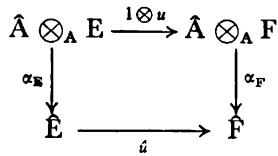
\includegraphics[keepaspectratio]{images/part002_24f0cc04.jpg}}

is commutative. Finally, it follows from § 2, no. 12, Proposition 16 that, if E is finitely generated, the homomorphism \(\alpha_{\mathbb{E}}\) is surjective.

THEOREM 3. Let A be a commutative Noetherian ring, m an ideal of A and E, F, G three finitely generated A-modules. Then:

\begin{enumerate}
\def\labelenumi{(\roman{enumi})}
\item
  If \(E \xrightarrow{u} F \xrightarrow{v} G\) is an exact sequence of A-linear mappings, the sequence \(\hat{E} \xrightarrow{\hat{u}} \hat{F} \xrightarrow{\hat{v}} \hat{G}\) obtained by passing to the Hausdorff completions (with respect to the m-adic topologies) is exact.
\item
  The canonical \(\hat{\mathbf{A}}\) -linear mapping \(\alpha_{\mathbf{E}}: \hat{\mathbf{A}} \otimes_{\mathbf{A}} \mathbf{E} \to \hat{\mathbf{E}}\) is bijective.
\item
  The A-module \(\hat{\mathbf{A}}\) is flat.
\end{enumerate}

We have seen that u and v are strict morphisms of topological groups (no. 2, Corollary to Theorem 2). Assertion (i) then follows from § 2, no. 12, Lemma 2. Assertion (ii) is obvious when E = A and the case where E is a free finitely generated A-module can be immediately reduced to that. In the general case, E admits a finite presentation

\[
\mathrm{L} \xrightarrow {u} \mathrm{L} ^ {\prime} \xrightarrow {v} \mathrm{E} \longrightarrow 0
\]

(Chapter I, § 2, no. 8, Lemma 8). We derive a commutative diagram

\pandocbounded{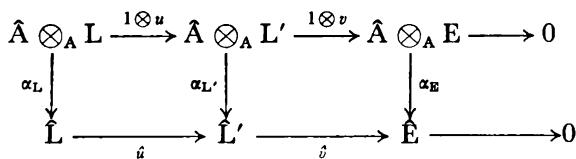
\includegraphics[keepaspectratio]{images/part002_14bc27b3.jpg}}

The first row is exact (Chapter I, § 2, no. 1, Lemma 1) and so is the second by (i). We already know that \(\alpha_{\mathrm{E}}\) is surjective (§ 2, no. 12, Proposition 16); on the other hand, as \(\alpha_{\mathrm{L}}\) and \(\alpha_{\mathrm{L}'}\) are bijective and \(1 \otimes v\) is surjective, \(\alpha_{\mathrm{E}}\) is injective by virtue of Chapter I, § 1, no. 4, Corollary 2 to Proposition 2; this shows (ii).

Then it follows from (i) and (ii) that, if \(a\) is an ideal of \(A\) (necessarily finitely generated), the canonical mapping \(\hat{A} \otimes_{A} a \to \hat{A}\) is injective, being the composition of \(\hat{a} \to \hat{A}\) and \(\alpha_{E}\) , which proves that \(\hat{A}\) is a flat A-module (Chapter I, § 2, no. 3, Proposition 1).

Under the conditions of Theorem 3 \(\hat{\mathbf{A}}\otimes_{\mathbf{A}}\mathbf{E}\) is often identified with \(\hat{\mathbf{E}}\) by means of the canonical mapping \(\alpha_{\mathbf{E}}\) . If \(u\colon \mathbf{E}\to \mathbf{F}\) is a homomorphism of finitely generated A-modules, \(\hat{u}\colon \hat{\mathbf{E}}\to \hat{\mathbf{F}}\) is then identified with \(1\otimes u\) by virtue of the commutativity of diagram (4).

COROLLARY 1. Let A be a commutative Noetherian ring, m an ideal of A, E a finitely generated A-module and F and G two submodules of E. Let A, E, F, G be given the m-adic topologies and let i be the canonical mapping from E to Ê. Then:

\[
\begin{array}{r l} \hat {\mathbf {F}} = \hat {\mathbf {A}}. i (\mathbf {F}), & (\mathbf {F} + \mathbf {G}) ^ {\wedge} = \hat {\mathbf {F}} + \hat {\mathbf {G}}, \\ & (\mathbf {F} \cap \mathbf {G}) ^ {\wedge} = \hat {\mathbf {F}} \cap \hat {\mathbf {G}}, \\ & (\mathbf {F}: \mathbf {G}) ^ {\wedge} = \hat {\mathbf {F}}: \hat {\mathbf {G}}. \end{array}
\]

Moreover, if a and b are two ideals of A and c = ab, \(\hat{c} = \hat{ab}\) .

By Theorem 3, \(\hat{\mathbf{E}}\) , \(\hat{\mathbf{F}}\) , \(\hat{\mathbf{G}}\) are canonically identified with \(\hat{\mathbf{A}} \otimes_{\mathbf{A}} \mathbf{E}\) , \(\hat{\mathbf{A}} \otimes_{\mathbf{A}} \mathbf{F}\) , \(\hat{\mathbf{A}} \otimes_{\mathbf{A}} \mathbf{G}\) , which establishes the first two formulae. The third and fourth follow respectively from Chapter I, § 2, no. 6, Proposition 6 and no. 10, Proposition 12. Finally, as \(\hat{\mathbf{a}} = \hat{\mathbf{A}}i(\mathfrak{a})\) , \(\hat{\mathfrak{b}} = \hat{\mathbf{A}}i(\mathfrak{b})\) , \(\hat{\mathfrak{c}} = \hat{\mathbf{A}}i(\mathfrak{c})\) ,

\[
\hat {\mathfrak {c}} = \hat {\mathrm{A}} i (\mathfrak {a b}) = \hat {\mathrm{A}} i (\mathfrak {a}) i (\mathfrak {b}) = \hat {\mathfrak {a b}}.
\]

COROLLARY 2. Let A be a commutative Noetherian ring, m an ideal of A and \(\hat{\mathbf{A}}\) the Hausdorff completion of A with respect to the m-adic topology. If an element \(a \in \mathbf{A}\) is not a divisor of 0 in A, its canonical image \(a'\) in \(\hat{\mathbf{A}}\) is not a divisor of 0 in \(\hat{\mathbf{A}}\) .

As \(\hat{\mathbf{A}}\) is a flat A-module, the corollary is a special case of Chapter I, § 2, no. 4, Proposition 3 (i).

COROLLARY 3. If A is a commutative Noetherian ring, the ring of formal power series A{[}{[}X₁, \ldots, Xₙ{]}{]} is a flat A-module.

It is the completion of the polynomial ring

\[
\mathbf {B} = \mathbf {A} [ \mathbf {X} _ {1}, \dots , \mathbf {X} _ {n} ]
\]

with respect to the m-adic topology, where m is the set of polynomials with no constant term (§ 2, no. 12, Example 1); as B is Noetherian (§ 2, no. 10, Corollary 2 to Theorem 2), A{[}{[}X₁, \ldots, Xₙ{]}{]} is a flat B-module by Theorem 3 and, as B is free A-module, A{[}{[}X₁, \ldots, Xₙ{]}{]} is a flat A-module (Chapter I, § 2, no. 7, Corollary 3 to Proposition 8).

PROPOSITION 8. Let A be a commutative Noetherian ring, m an ideal of A, \(\hat{A}\) the Hausdorff completion of A with respect to the m-adic topology and j the canonical mapping from A to \(\hat{A}\) . The :

\begin{enumerate}
\def\labelenumi{(\roman{enumi})}
\item
  \(\hat{\mathbf{A}}\) is a Zariski ring and \(\hat{\mathfrak{m}} = \hat{\mathbf{A}}.j(\mathfrak{m})\) is a defining ideal of \(\hat{\mathbf{A}}\) .
\item
  The mapping \(\mathfrak{n} \mapsto \hat{\mathfrak{n}} = \hat{\mathbf{A}}.j(\mathfrak{n})\) is a bijection of the set of maximal ideals of \(\mathbf{A}\) containing \(\mathfrak{m}\) onto the set of maximal ideals of \(\hat{\mathbf{A}}\) and \(\mathfrak{q} \mapsto j^{-1}(\mathfrak{q})\) is the inverse bijection.
\item
  Let \(\mathfrak{n}\) be a maximal ideal of \(\mathbf{A}\) containing \(\mathfrak{m}\) . The homomorphism \(j': \mathbf{A}_{\mathfrak{n}} \to \hat{\mathbf{A}}_{\hat{\mathfrak{n}}}\) derived from \(j\) is injective; if \(\mathbf{A}_{\mathfrak{n}}\) is identified by means of \(j\) with a subring of \(\hat{\mathbf{A}}_{\hat{\mathfrak{n}}}\) , the \((\mathfrak{n}\mathbf{A}_{\mathfrak{n}})\) -adic topology on \(\mathbf{A}_{\mathfrak{n}}\) is induced by the \(\hat{\mathfrak{n}}\) -adic topology on \(\hat{\mathbf{A}}_{\hat{\mathfrak{n}}}\) and \(\mathbf{A}_{\mathfrak{n}}\) is dense in \(\hat{\mathbf{A}}_{\hat{\mathfrak{n}}}\) with the \(\hat{\mathfrak{n}}\) -adic topology.
\end{enumerate}

Let us show (i). As \(\mathfrak{m}\) is a finitely generated ideal, \((\mathfrak{m}^n)^{\circ} = (\hat{\mathfrak{m}})^n = \mathfrak{m}^n\hat{\mathbf{A}}\) (§ 2, no. 12, Corollary 2 to Proposition 16) and the topology on \(\hat{\mathbf{A}}\) is the \(\hat{\mathfrak{m}}\) -adic topology. As \(\hat{\mathbf{A}}/\hat{\mathfrak{m}}\) is isomorphic to \(\mathbf{A}/\mathfrak{m}\) , it is a Noetherian ring and \(\hat{\mathfrak{m}} = \mathfrak{m}\hat{\mathbf{A}}\) is a finitely generated \(\hat{\mathbf{A}}\) -module and therefore \(\hat{\mathbf{A}}\) is Noetherian (§ 2, no. 10, Corollary 5 to Theorem 2); finally, as \(\hat{\mathbf{A}}\) is Hausdorff and complete with respect to the \(\hat{\mathfrak{m}}\) -adic topology, \(\hat{\mathbf{A}}\) is a Zariski ring (no. 3, Example 1).

Assertion (ii) follows immediately from the fact that the canonical homomorphism \(A/m \rightarrow \hat{A}/\hat{m}\) derived from j is bijective and the fact that every maximal ideal of \(\hat{A}\) contains \(\hat{m}\) , since \(\hat{A}\) is a Zariski ring and the Jacobson radical of \(\hat{A}\) then contains \(\hat{m}\) (no. 3, Proposition 6).

Finally let us prove (iii). As \(\mathfrak{n} = j^{-1}(\hat{\mathfrak{n}}), j(\mathbf{A} - \mathfrak{n}) \subset \hat{\mathbf{A}} - \hat{\mathfrak{n}}\) and \(j\) certainly defines a homomorphism \(j' \colon \mathbf{A}_{\mathfrak{n}} \to \hat{\mathbf{A}}_{\hat{\mathfrak{n}}}\) (Chapter II, § 2, no. 1, Proposition 2). Let us show that \(j'\) is injective; let \(a \in \mathbf{A}, s \in \mathbf{A} - \mathfrak{n}\) be such that

\[
j ^ {\prime} (a / s) = j (a) / j (s) = 0;
\]

then there exists \(s' \in \hat{\mathbf{A}} - \hat{\mathfrak{n}}\) such that \(s'j(a) = 0\) (Chapter II, §2, no. 1, Remark 3) and the annihilator of \(j(a)\) in \(\hat{\mathbf{A}}\) is therefore not contained in \(\hat{\mathfrak{n}}\) . Now, if \(\mathfrak{b}\) is the annihilator of \(a\) in \(\mathbf{A}\) , the annihilator of \(j(a)\) in \(\hat{\mathbf{A}}\) is \(\mathfrak{b}\) (Corollary 1 to Theorem 3); hence \(\mathfrak{b} \not\subset \mathfrak{n}\) , which shows that \(a / s = 0\) .

Moreover, there is a commutative diagram

\[
\begin{array}{c} \mathrm{A} / \mathfrak {n} ^ {k} \longrightarrow \mathrm{A} _ {\mathfrak {n}} / (\mathfrak {n} \mathrm{A} _ {\mathfrak {n}}) ^ {k} \\ \stackrel {{h}} {{\downarrow}} \qquad \qquad \qquad \qquad \qquad \qquad \qquad \qquad \qquad \qquad \qquad \qquad \qquad \qquad \qquad \qquad \qquad \qquad \qquad \qquad \qquad \qquad \qquad \hat {\mathrm{A}} / \hat {\mathfrak {n}} ^ {k} \longrightarrow \hat {\mathrm{A}} _ {\hat {\mathfrak {n}}} / (\hat {\mathfrak {n}} \hat {\mathrm{A}} _ {\hat {\mathfrak {n}}}) ^ {k} \end{array}\tag{5}
\]

where \(h\) and \(h'\) are derived from \(j\) and \(j'\) respectively and the horizontal arrows are the canonical isomorphisms of Chapter II, § 3, no. 3, Proposition 9. As \(n^k\) is an open ideal of A (since it contains \(m^k\) ), \(h\) is bijective and hence so is \(h'\) . This shows first that \((\mathfrak{n}\mathbf{A}_{\mathfrak{n}})^k = j'((\hat{\mathfrak{n}}\hat{\mathbf{A}}_{\hat{\mathfrak{n}}})^k)\) and hence the topology on \(\mathbf{A}_{\mathfrak{n}}\) is induced by that on \(\hat{\mathbf{A}}_{\hat{\mathfrak{n}}}\) ; moreover, \(\hat{\mathbf{A}}_{\hat{\mathfrak{n}}} = \mathbf{A}_{\mathfrak{n}} + (\hat{\mathfrak{n}}\hat{\mathbf{A}}_{\hat{\mathfrak{n}}})^k\) for all \(k > 0\) and hence \(\mathbf{A}_{\mathfrak{n}}\) is everywhere dense in \(\hat{\mathbf{A}}_{\hat{\mathfrak{n}}}\) .

COROLLARY. Let A be a Noetherian local (resp. semi-local) ring and m its Jacobson radical. Then \(\hat{A}\) is a Noetherian local (resp. semi-local) ring whose Jacobson radical is \(\hat{m}\) .

\(\hat{\mathbf{A}}\) is Noetherian by Proposition 8 (i) and the rest follows from Proposition 8 (ii) and the third formula in Corollary 1 to Theorem 3.

\subsection{The completion of a Zariski ring}

PROPOSITION 9. Let A be a commutative Noetherian ring and m an ideal of A; let A be given the m-adic topology. For \(\hat{\mathbf{A}}\) to be a faithfully flat A-module, it is necessary and sufficient that A be a Zariski ring.

For every finitely generated A-module M, the canonical mapping \(M \to M \otimes_{A} \hat{A}\) is identified with the canonical mapping \(M \to \hat{M}\) from M to its Hausdorff completion with respect to the m-adic topology (no. 4, Theorem 3) and the kernel of this mapping is then the closure of \(\{0\}\) in M with respect to this topology. As we already know that \(\hat{A}\) is a flat A-module (no. 4, Theorem 3), the proposition follows from the characterization of faithfully flat modules (Chapter I, §3, no. 1, Proposition 1 (b)) and the characterization of Zariski rings (no. 3, Proposition 6).

If A is a Zariski ring and E is a finitely generated A-module, we may (by virtue of Proposition 9) identify E with a subset of \(\hat{E}\) by means of the canonical mapping \(j_{E}: E \to \hat{E}\) . With this identification:

COROLLARY 1. Let A be a Zariski ring, E a finitely generated A-module and F a submodule of E. Then \(\mathbf{F} = \hat{\mathbf{F}} \cap \mathbf{E} = (\hat{\mathbf{A}}\mathbf{F}) \cap \mathbf{E}\) .

This is a special case of Chapter I, § 3, no. 5, Proposition 10 (ii) and it also follows from no. 3, Proposition 6.

COROLLARY 2. Let A be a Zariski ring and E a finitely generated A-module. If \(\hat{\mathbf{E}}\) is a free \(\hat{\mathbf{A}}\) -module, E is a free A-module.

Let \(\mathfrak{m}\) be a defining ideal of \(\mathbf{A}\) , which is therefore contained in the Jacobson radical of \(\mathbf{A}\) . We apply the criterion of Chapter II, § 3, no. 5, Proposition 5: the canonical mapping \(j_{\mathrm{E}}: \mathrm{E} \to \hat{\mathrm{E}}\) defines a bijection \(i_{\mathrm{E}}: \mathrm{E} / \mathfrak{m}\mathrm{E} \to \hat{\mathrm{E}} / (\mathfrak{m}\mathrm{E})^{\wedge}\) ; similarly the canonical mapping \(j_{\mathrm{A}}: \mathrm{A} \to \hat{\mathrm{A}}\) defines a bijection \(i_{\mathrm{A}}: \mathrm{A} / \mathfrak{m} \to \hat{\mathrm{A}} / \hat{\mathfrak{m}}\) , which is a ring isomorphism. Then \((\mathfrak{m}\mathrm{E})^{\wedge} = \hat{\mathrm{A}}. \mathfrak{m}\mathrm{E} = \hat{\mathfrak{m}}\hat{\mathrm{E}}\) (no. 4, Theorem 3), so that \(\hat{\mathrm{E}} / (\mathfrak{m}\mathrm{E})^{\wedge}\) is given an \((\hat{\mathrm{A}} / \hat{\mathfrak{m}})\) -module structure and hence (by means of \(i_{\mathrm{A}}\) ) an \((\mathrm{A} / \mathfrak{m})\) -module structure. It is immediate that \(i_{\mathrm{E}}\) is \((\mathrm{A} / \mathfrak{m})\) -linear, so that it is an \((\mathrm{A} / \mathfrak{m})\) -module isomorphism. As \(\hat{\mathrm{E}} / \hat{\mathfrak{m}}\hat{\mathrm{E}}\) is a free \((\hat{\mathrm{A}} / \hat{\mathfrak{m}})\) -module, \(\mathrm{E} / \mathfrak{m}\mathrm{E}\) is a free \((\mathrm{A} / \mathfrak{m})\) -module.

On the other hand, let \(v: \mathfrak{m} \otimes_{\mathbf{A}} \mathbf{E} \to \mathbf{E}\) be the canonical homomorphism; as \((\mathfrak{m} \otimes_{\mathbf{A}} \mathbf{E}) \otimes_{\mathbf{A}} \hat{\mathbf{A}}\) is canonically identified with \(\hat{\mathfrak{m}} \otimes_{\mathbf{A}} \hat{\mathbf{E}}\) and \(\mathbf{E} \otimes_{\mathbf{A}} \hat{\mathbf{A}}\) with \(\hat{\mathbf{E}}\) (no. 4, Theorem 3), the hypothesis that \(\hat{\mathbf{E}}\) is a free \(\hat{\mathbf{A}}\) -module implies that the homomorphism \(v \otimes 1: \hat{\mathfrak{m}} \otimes_{\hat{\mathbf{A}}} \hat{\mathbf{E}} \to \hat{\mathbf{E}}\) is injective. As \(\hat{\mathbf{A}}\) is a faithfully flat A-module (Proposition 9), we conclude that \(v\) is injective (Chapter I, § 3, no. 1, Proposition 2) and the conditions for applying the above mentioned criterion are indeed fulfilled.

COROLLARY 3. Let A be a Zariski ring such that \(\hat{\mathbf{A}}\) is an integral domain and let \(\mathfrak{a}\) be an ideal of A. If the ideal \(\mathfrak{a}\hat{\mathbf{A}}\) of \(\hat{\mathbf{A}}\) is principal, \(\mathfrak{a}\) is principal. This is a special case of Corollary 2.

COROLLARY 4. Let A be a Zariski ring such that \(\hat{\mathbf{A}}\) is an integral domain, L the field of fractions of \(\hat{\mathbf{A}}\) and \(\mathbf{K} \subset \mathbf{L}\) the field of fractions of A; then \(\hat{\mathbf{A}} \cap \mathbf{K} = \mathbf{A}\) .

Clearly \(\mathbf{A} \subset \hat{\mathbf{A}} \cap \mathbf{K}\) ; on the other hand, if \(x \in \hat{\mathbf{A}} \cap \mathbf{K}\) , then \(\hat{\mathbf{A}}x \subset \hat{\mathbf{A}}\) and hence, as \(\hat{\mathbf{A}}x = \hat{\mathbf{A}} \otimes_{\mathbf{A}} (\mathbf{A}x)\) (no. 4, Theorem 3), \(\hat{\mathbf{A}} \otimes_{\mathbf{A}} ((\mathbf{A}x + \mathbf{A}) / \mathbf{A}) = 0\) . As \(\hat{\mathbf{A}}\) is a faithfully flat A-module (Proposition 9), we deduce that \(\mathbf{A}x \subset \mathbf{A}\) , whence \(x \in \mathbf{A}\) .

COROLLARY 5. Let A be a commutative Noetherian ring, E, F two finitely generated A-modules and u: E → F an A-homomorphism. For every maximal ideal m of A, let A(m) (resp. E(m), F(m)) denote the Hausdorff completion of A (resp. E, F) with respect to the m-adic topology and u(m): E(m) → F(m) the corresponding homomorphism to u. For u to be injective (resp. surjective, bijective, zero), it is necessary and sufficient that u(m) be so for every maximal ideal m of A.

We know that for \(u\) to be injective (resp. surjective, bijective, zero), it is necessary and sufficient that \(u_{\mathfrak{m}}: \mathrm{E}_{\mathfrak{m}} \to \mathrm{F}_{\mathfrak{m}}\) be so for every maximal ideal \(\mathfrak{m}\) of \(\mathbf{A}\) (Chapter II, § 3, no. 3, Theorem 1). We now note that \(\mathbf{A}_{\mathfrak{m}}\) is a Noetherian local ring (Chapter II, § 2, no. 4, Corollary 2 to Proposition 10) and hence a Zariski ring and there is a canonical A-algebra isomorphism \(\hat{\mathbf{A}}_{\mathfrak{m}} \to \mathbf{A}(\mathfrak{m})\) (§ 2, no. 13, Proposition 18). On the other hand (beginning of no. 4), there is a commutative diagram

\[
\begin{array}{l} \mathrm{E} _ {\mathfrak {m}} \otimes_ {\mathbf {A} _ {\mathfrak {m}}} \mathrm{A} (\mathfrak {m}) \longrightarrow \mathrm{E} \otimes_ {\mathbf {A}} \mathrm{A} (\mathfrak {m}) \longrightarrow \mathrm{E} (\mathfrak {m}) \\ u _ {\mathfrak {m}} \otimes 1 \Biggl \downarrow \qquad \qquad \qquad \qquad \Biggl \downarrow u \otimes 1 \qquad \qquad \Biggl \downarrow u (\mathfrak {m}) \\ \mathrm{F} _ {\mathfrak {m}} \otimes_ {\mathbf {A} _ {\mathfrak {m}}} \mathrm{A} (\mathfrak {m}) \longrightarrow \mathrm{F} \otimes_ {\mathbf {A}} \mathrm{A} (\mathfrak {m}) \longrightarrow \mathrm{F} (\mathfrak {m}) \end{array}
\]

where the horizontal arrows on the left arise from the associativity of the tensor product and the isomorphisms \(E_{m} \rightarrow E \otimes_{A} A_{m}\) , \(F_{m} \rightarrow F \otimes_{A} A_{m}\) ; as E and F are finitely generated A-modules, it follows from no. 4, Theorem 3 that the rows of this diagram consist of isomorphisms; thus we are reduced to proving that \(u_{m}\) being injective (resp. surjective, bijective, zero) is equivalent to \(u_{m} \otimes 1\) being so. But this follows from the fact that \(\hat{A}_{m}\) (and hence also \(A(m)\) ) is a faithfully flat \(A_{m}\) -module by Proposition 9 (Chapter I, § 3, no. 1, Propositions 1 and 2).

PROPOSITION 10. Let A, B be two Zariski rings, \(\hat{A}\) , \(\hat{B}\) their completions, \(f\colon A\to B\) a continuous ring homomorphism and \(\hat{f}\colon\hat{A}\to\hat{B}\) the homomorphism obtained from \(f\) by passing to the completions; if \(\hat{f}\) is bijective, the A-module B is faithfully flat.

As A and B are Hausdorff, the hypothesis that \(\hat{f}\) is bijective implies first that \(f\) is injective. Identifying (algebraically) A with \(f(A)\) by means of \(f\) and \(\hat{A}\) with \(\hat{B}\) by means of \(\hat{f}\) , we then obtain the inclusions \(A \subset B \subset \hat{A} = \hat{B}\) ; we know that \(\hat{A}\) is a faithfully flat A-module and a faithfully flat B-module (Proposition 9); we conclude that B is a faithfully flat A-module (Chapter I, § 3, no. 4, Remark 2).

PROPOSITION 11. Let A be a Noetherian local ring, m its maximal ideal, \(\hat{\mathbf{A}}\) its m-adic completion and B a ring such that \(\mathbf{A} \subset \mathbf{B} \subset \hat{\mathbf{A}}\) . Suppose that B is a Noetherian local ring whose maximal ideal n satisfies the relation \(n = mB\) . Then

\[
\mathfrak {n} ^ {k} = \mathfrak {m} ^ {k} \mathrm{B} = \hat {\mathfrak {m}} ^ {k} \cap \mathrm{B}
\]

for all \(k \geqslant 1\) , the \(\mathfrak{n}\) -adic topology on \(\mathbf{B}\) is induced by the \(\hat{\mathfrak{m}}\) -adic topology on \(\hat{\mathbf{A}}\) , \(\mathbf{B}\) is a faithfully flat \(\mathbf{A}\) -module and there is an isomorphism of \(\hat{\mathbf{A}}\) onto the \(\mathfrak{n}\) -adic completion \(\hat{\mathbf{B}}\) of \(\mathbf{B}\) , which extends the canonical injection \(\mathbf{A} \to \mathbf{B}\) .

It is sufficient to verify the relation \(n^{k} = \hat{m}^{k} \cap B\) , for, as B is dense in \(\hat{A}\) and the n-adic topology is induced by the \(\hat{m}\) -adic topology, the last assertion will follow from General Topology, Chapter II, §3, no. 9, Corollary 1 to Proposition 18 and the last but one from Proposition 10. The injection \(j_{A}: A \to \hat{A}\) (resp. \(j_{B}: B \to \hat{A}\) ) defines by taking quotients an injective homomorphism

\[
i _ {\mathbf {A}} \colon \mathrm{A} / (\hat {\mathfrak {m}} \cap \mathrm{A}) \rightarrow \hat {\mathrm{A}} / \hat {\mathfrak {m}}
\]

(resp. \(i_{B}\) : B/(m ∩ B) → Â/m). We know that m ∩ A = m and that \(i_{A}\) is bijective, hence \(i_{B}\) is bijective, which shows that B/(m ∩ B) is a field, hence that m ∩ B is a maximal ideal of B and therefore m ∩ B = n.~As \(\hat{A} = A + \hat{m}\) , \(B = A + n = A + mB\) ; by induction on k we deduce that

\[
\mathbf {B} = \mathbf {A} + \mathfrak {m} ^ {k} \mathbf {B} = \mathbf {A} + \mathfrak {n} ^ {k}
\]

for all \(k > 1\) . As \(\mathfrak{n}^k \subset \hat{\mathfrak{m}}^k \cap \mathbf{B}\) , it is sufficient to show that \(\hat{\mathfrak{m}}^k \cap \mathbf{B} \subset \mathfrak{n}^k\) ; if \(b \in \hat{\mathfrak{m}}^k \cap \mathbf{B}\) , we may write \(b = a + z\) where \(a \in \mathbf{A}\) , \(z \in \mathfrak{n}^k\) ; whence

\[
a = b - z \in \hat {\mathfrak {m}} ^ {k} \cap \mathrm{A} = \mathfrak {m} ^ {k} \subset \mathfrak {n} ^ {k}
\]

and \(b \in \mathfrak{n}^k\) .

* An important case where this applies is the following: B is the ring of integral series in n variables over a complete valued field, which converge in the neighbourhood of 0, A is the local ring

\[
\mathrm{K} [ \mathrm{X} _ {1}, \dots , \mathrm{X} _ {n} ] _ {\mathfrak {p}}
\]

where p is the maximal ideal consisting of the polynomials with no constant term and \(\hat{A}\) is the ring of formal power series \(K[[X_{1},\ldots,X_{n}]]\) . *

\pandocbounded{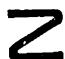
\includegraphics[keepaspectratio]{images/part002_72a4a9a7.jpg}}

Remark. A local ring B such that \(A \subset B \subset \hat{A}\) , whose maximal ideal n is equal to mB and whose n-adic topology is induced by the m-adic topology on \(\hat{A}\) , is not necessarily Noetherian (Exercise 14).

PROPOSITION 12. Let A be a commutative Noetherian ring, m an ideal of A, S the multiplicative subset \(1 + m\) of A and E a finitely generated A-module. Under these conditions:

\begin{enumerate}
\def\labelenumi{(\roman{enumi})}
\item
  \(\mathbf{S}^{-1}\mathbf{A}\) is a Zariski ring with the \((\mathbf{S}^{-1}\mathfrak{m})\) -adic topology.
\item
  The canonical mapping \(f \colon \mathbf{E} \to \mathbf{S}^{-1}\mathbf{E}\) is continuous if \(\mathbf{E}\) is given the \(\mathfrak{m}\) -adic topology and \(\mathbf{S}^{-1}\mathbf{E}\) the \((\mathbf{S}^{-1}\mathfrak{m})\) -adic topology and \(\hat{f} \colon \hat{\mathbf{E}} \to (\mathbf{S}^{-1}\mathbf{E})^{\wedge}\) is an isomorphism.
\end{enumerate}

Every element of \(1 + (\mathbf{S}^{-1}\mathfrak{m})\) is of the form

\[
1 + (m / \left(1 + m ^ {\prime}\right)) = (1 + m + m ^ {\prime}) / (1 + m)
\]

where \(m \in m\) and \(m' \in m\) ; it is therefore invertible in \(S^{-1}A\) , which proves that \(S^{-1}m\) is contained in the Jacobson radical of \(S^{-1}A\) ; as \(S^{-1}A\) is Noetherian (Chapter II, §2, no. 4, Corollary 2 to Proposition 10), \(S^{-1}A\) is a Zariski ring with the \((\mathrm{S}^{-1}\mathrm{m})\) -adic topology, which proves (i). Let us show (ii). For all n \textgreater{} 0,

\[
\bar {f} ^ {- 1} ((S ^ {- 1} m) ^ {n} E) = \bar {f} ^ {- 1} (S ^ {- 1} (m ^ {n} E)) = m ^ {n} E:
\]

for clearly first of all \(f(\mathfrak{m}^n\mathrm{E}) \subset \mathrm{S}^{-1}\mathfrak{m}^n\mathrm{E}\) ; conversely, let \(x\) be an element of \(f^{-1}(\mathrm{S}^{-1}\mathfrak{m}^n\mathrm{E})\) ; then there exist elements \(m', m''\) of \(\mathfrak{m}\) and \(x'' \in \mathfrak{m}^n\mathrm{E}\) such that \((1 + m')((1 + m'')x - x'') = 0\) , whence \((1 - m)x = x'\) , where

\[
m = - \left(m ^ {\prime} + m ^ {\prime \prime} + m ^ {\prime} m ^ {\prime \prime}\right) \in \mathfrak {m}
\]

and \(x' = (1 + m')x'' \in \mathfrak{m}^n\mathrm{E}\) ; we conclude that

\[
x = (1 + m + \dots + m ^ {n - 1}) x ^ {\prime} + m ^ {n} x \in \mathfrak {m} ^ {n} \mathrm{E}.
\]

This proves that \(f\) is a strict morphism. Moreover, the kernel of \(f\) , which is the set of \(x \in \mathbf{E}\) for which there exists some \(s \in \mathbf{S}\) such that \(sx = 0\) , is identical with the kernel of the canonical mapping \(j: \mathbf{E} \to \hat{\mathbf{E}}\) (no. 2, Proposition 5). Then there is a topological isomorphism \(f_0: j(\mathbf{E}) \to f(\mathbf{E})\) such that \(f = f_0 \circ j\) ; as \(j\) is a topological isomorphism, the problem reduces to verifying that \(f(\mathbf{E})\) is dense in \(\mathbf{S}^{-1}\mathbf{E}\) . Now every element of \(\mathbf{S}^{-1}\mathbf{E}\) may be written as \(x / (1 - m)\) , where \(m \in \mathfrak{m}\) , and it is immediately verified that

\[
x / (1 - m) \equiv ((1 + m + \dots + m ^ {n - 1}) x) / 1 (\mathrm{mod.} \mathrm{S} ^ {- 1} \mathrm{m} ^ {n} \mathrm{E})
\]

which completes the proof.

\section{LIFTING IN COMPLETE RINGS}

\subsection{Strongly relatively prime polynomials}

Let R be a commutative ring. Two elements x, y of R are called strongly relatively prime if the principal ideals Rx and Ry are relatively prime, in other words (Chapter II, § 1, no. 2) if \(\mathbf{R}x + \mathbf{R}y = \mathbf{R}\) ; it amounts to the same to say that there exist two elements \(a, b\) of \(\mathbf{R}\) such that \(ax + by = 1\) .

LEMMA 1 (``Euclid's Lemma''). Let \(x, y\) be two strongly relatively prime elements of \(\mathbf{R}\) ; if \(z \in \mathbf{R}\) is such that \(x\) divides \(yz\) , then \(x\) divides \(z\) .

If \(1 = ax + by\) , then \(z = x(az) + (yz)b\) .

If \(x\) and \(y\) are strongly relatively prime in \(\mathbf{R}\) , then

\[
\mathrm{R} x y = (\mathrm{R} x) \cap (\mathrm{R} y)
\]

(Chapter II, § 1, no. 2, Proposition 5); if R is an integral domain, two strongly relatively prime elements then have an lcm equal to their product (Algebra, Chapter VI, § 1, no. 8) and are therefore relatively prime in the sense of Algebra, Chapter VI, § 1, no. 12. Conversely, if R is a principal ideal domain, two relatively prime elements are also strongly relatively prime, as follows from Bezout's identity (Algebra, Chapter VII, § 1, no. 2, Theorem 1).

For polynomial rings there is the following result:

PROPOSITION 1. Let A be a commutative ring and P and P' two strongly relatively prime polynomials in A{[}X{]}. Suppose that P is monic and of degree s. Then every polynomial T in A{[}X{]} may be written uniquely in the form

\[
\mathrm{T} = \mathrm{PQ} + \mathrm{P} ^ {\prime} \mathrm{Q} ^ {\prime}\tag{1}
\]

where \(\mathbf{Q} \in \mathbf{A}[\mathbf{X}]\) , \(\mathbf{Q}' \in \mathbf{A}[\mathbf{X}]\) and \(\deg(\mathbf{Q}') < s\) .

If further \(\deg (\mathbf{T})\leqslant t\) and \(\deg (\mathbf{P}^{\prime})\leqslant t - s\) , then \(\deg (\mathbf{Q})\leqslant t - s\)

As \(\mathbf{P}\) is monic, \(\mathrm{PR} \neq 0\) for every polynomial \(\mathbf{R} \neq 0\) of \(\mathbf{A}[\mathbf{X}]\) and in this case \(\deg(\mathrm{PR}) = s + \deg(\mathbf{R})\) .

Let \(\mathbf{T}\) be any polynomial in A{[}X{]}. As the ideal generated by P and \(\mathbf{P}'\) is the whole of A{[}X{]}, there exist polynomials \(\mathbf{Q}_1\) and \(\mathbf{Q}_1'\) such that

\[
\mathrm{T} = \mathrm{PQ} _ {1} + \mathrm{P} _ {1} ^ {\prime} \mathrm{Q} _ {1} ^ {\prime};
\]

as P is monic of degree s, Euclidean division (Algebra, Chapter IV, § 1, no. 5) shows that there exist two polynomials Q', Q'\,' such that Q'\_1 = PQ'\,' + Q' where deg(Q') \textless{} s; then we deduce that

\[
\mathrm{T} = \mathrm{PQ} _ {1} + \mathrm{P} ^ {\prime} (\mathrm{PQ} ^ {\prime \prime} + \mathrm{Q} ^ {\prime}) = \mathrm{PQ} + \mathrm{P} ^ {\prime} \mathrm{Q} ^ {\prime}
\]

where \(Q = Q_{1} + P'Q''\) . To show the uniqueness of formula (1), it is sufficient to prove that the relations

\[
0 = \mathrm{PQ} + \mathrm{P} ^ {\prime} \mathrm{Q} ^ {\prime}, \quad \deg (\mathrm{Q} ^ {\prime}) <   s\tag{2}
\]

imply \(Q = Q' = 0\) . Now, if (2) holds, \(P\) divides \(-PQ = P'Q'\) and, as \(P\) and

\(P'\) are strongly relatively prime, \(P\) divides \(Q'\) by Lemma 1; if \(Q' \neq 0\) , there would exist a polynomial \(S \neq 0\) such that \(Q' = PS\) , whence

\[
\deg (\mathbf {Q} ^ {\prime}) = s + \deg (\mathbf {S}) \geqslant s,
\]

which is a contradiction. We conclude that \(Q' = 0\) , whence PQ = 0 and finally Q = 0 by the remark at the beginning.

Finally, suppose that \(\deg(T) \leqslant t\) and \(\deg(P') \leqslant t - s\) ; with the polynomial \(T\) in the form (1),

\[
\deg (\mathrm{P} ^ {\prime} \mathrm{Q} ^ {\prime}) \leqslant \deg (\mathrm{P} ^ {\prime}) + \deg (\mathrm{Q} ^ {\prime}) <   s + \deg (\mathrm{P} ^ {\prime}) \leqslant t
\]

and therefore

\[
s + \deg (Q) = \deg (P Q) = \deg (T - P ^ {\prime} Q ^ {\prime}) \leqslant t
\]

whence \(\deg (\mathbb{Q})\leqslant t - s.\)

Example. For a polynomial \(P \in A[X]\) to be strongly relatively prime to X - a (where \(a \in A\) ), it is necessary and sufficient that \(P(a)\) be invertible in A. For if P and X - a are strongly relatively prime, it follows from Proposition 1 that there exist \(c \in A\) and a polynomial \(Q \in A[X]\) such that \(cP + (X - a)Q = 1\) , whence \(cP(a) = 1\) and \(P(a)\) is invertible. Conversely, by Euclidean division

\[
\mathbf {P} = (\mathbf {X} - a) \mathbf {R} + \mathbf {P} (a)
\]

and, if \(\mathrm{P}(a)=b^{-1}\) , where \(b\in A\) , we deduce that \(1=b\mathrm{P}-b(\mathrm{X}-a)\mathrm{R}\) , which shows that P and X-a are strongly relatively prime.

Let A and B be two commutative rings and \(f\colon\mathbf{A}\to\mathbf{B}\) a ring homomorphism. If \(\mathbf{P}=\sum_{i\geqslant0}a_{i}\mathbf{X}^{i}\) is a formal power series in \(\mathbf{A}[[\mathbf{X}]]\) , let \(\bar{f}(\mathbf{P})\) denote the formal power series \(\sum_{i\geqslant0}f(a_{i})\mathbf{X}^{i}\) in \(\mathbf{B}[[\mathbf{X}]]\) . If \(\mathbf{P}\) is a polynomial, so is \(\bar{f}(\mathbf{P})\) and, if further \(\mathbf{P}\) is monic, then \(\bar{f}(\mathbf{P})\) is monic of the same degree as \(\mathbf{P}\) . Finally, \(\mathbf{P}\mapsto\bar{f}(\mathbf{P})\) is clearly a homomorphism of \(\mathbf{A}[[\mathbf{X}]]\) to \(\mathbf{B}[[\mathbf{X}]]\) which extends \(f\) and maps \(\mathbf{X}\) to \(\mathbf{X}\) . The notation \(\bar{f}\) will be constantly used in this sense in the rest of this paragraph.

PROPOSITION 2. Let A and B be two commutative rings, f a homomorphism from A to B and P, P' two polynomials in A{[}X{]}. If P and P' are strongly relatively prime in A{[}X{]}, then \(\bar{f}(\mathbf{P})\) and \(\bar{f}(\mathbf{P}')\) are strongly relatively prime in B{[}X{]}. The converse is true if \(f\) is surjective, if its kernel is contained in the Jacobson radical of A and if P is monic.

Suppose that P and \(P'\) are strongly relatively prime; then there exist polynomials Q, \(Q'\) in A{[}X{]} such that \(PQ + P'Q' = 1\) ; we deduce that

\[
\bar {f} (\mathbf {P}) \bar {f} (\mathbf {Q}) + \bar {f} (\mathbf {P} ^ {\prime}) \bar {f} (\mathbf {Q} ^ {\prime}) = 1,
\]

whence the first assertion. To show the second, let a denote the kernel of f;

let \(\mathbf{E} = \mathbf{A}[\mathbf{X}]\) and \(\mathbf{F}\) the ideal of \(\mathbf{E}\) generated by \(\mathbf{P}\) and \(\mathbf{P}'\) ; as \(f\) is surjective and \(\bar{f}(\mathbf{P})\) monic, Proposition 1 shows that for every polynomial \(\mathbf{T} \in \mathbf{A}[\mathbf{X}]\) there exist two polynomials \(\mathbf{Q}, \mathbf{Q}'\) in \(\mathbf{A}[\mathbf{X}]\) such that

\[
\bar {f} (\mathrm{T}) = \bar {f} (\mathrm{P}) \bar {f} (\mathrm{Q}) + \bar {f} (\mathrm{P} ^ {\prime}) \bar {f} (\mathrm{Q} ^ {\prime}),
\]

whence the relation \(E = F + aE\) . Now, E/F is a finitely generated A-module, for every polynomial is congruent mod. P to a polynomial of degree \(<\deg(P)\) , P being monic. As \(E/F = a(E/F)\) and a is contained in the Jacobson radical of A, Nakayama's Lemma shows that \(E/F = 0\) (Algebra, Chapter VIII, §6, no. 3, Corollary 2 to Proposition 6), which means that P and \(P'\) are strongly relatively prime.

\subsection{Restricted formal power series}

DEFINITION 1. A commutative topological ring A is said to be linearly topologized (and its topology is said to be linear) if there exists a fundamental system B of neighbourhoods of 0 consisting of ideals of A.

Note that in such a ring, the ideals \(\mathfrak{S} \in \mathcal{B}\) are open and closed (General Topology, Chapter III, § 2, no. 1, Corollary to Proposition 4). For all \(\mathfrak{S} \in \mathcal{B}\) , the quotient topological ring A/ \(\mathfrak{S}\) is then discrete; for \(\mathfrak{S} \in \mathcal{B}\) , \(\mathfrak{S}' \in \mathcal{B}\) , \(\mathfrak{S}' \subset \mathfrak{S}\) , let

\[
h _ {\mathfrak {S S} ^ {\prime}} \colon \mathrm{A} / \mathfrak {S} ^ {\prime} \rightarrow \mathrm{A} / \mathfrak {S}
\]

be the canonical mapping. We know (General Topology, Chapter III, § 7, no. 3) that \((\mathbf{A} / \mathfrak{S}, h_{\mathfrak{S}\mathfrak{S}'})\) is an inverse system of discrete rings (relative to the indexing set \(\mathcal{B}\) which is ordered by \(\supset\) and directed), whose inverse limit is a complete Hausdorff linearly topologized ring \(\tilde{\mathbf{A}}\) ; further (loc. cit., Proposition 2), a strict morphism \(i: \mathbf{A} \to \tilde{\mathbf{A}}\) is defined, whose kernel is the closure of \(\{0\}\) in \(\mathbf{A}\) and whose image is everywhere dense in \(\tilde{\mathbf{A}}\) , so that \(\tilde{\mathbf{A}}\) is canonically identified with the Hausdorff completion of \(\mathbf{A}\) .

DEFINITION 2. Given a commutative topological ring A, a formal power series

\[
\mathbf {T} = \sum_ {(n _ {i})} c _ {n _ {1} n _ {2} \dots n _ {p}} \mathbf {X} _ {1} ^ {n _ {1}} \mathbf {X} _ {2} ^ {n _ {2}} \dots \mathbf {X} _ {p} ^ {n _ {p}}
\]

in the ring \(\mathbf{A}[[\mathbf{X}_1,\ldots ,\mathbf{X}_p]]\) is called restricted if, for every neighbourhood \(\mathbf{V}\) of 0 in A, there is only a finite number of coefficients \(c_{n_1n_2\dots n_p}\) not belonging to \(\mathbf{V}\) (in other words, the family \((c_{n_1n_2\dots n_p})\) tends to 0 in A with respect to the filter of complements of finite subsets of \(\mathbf{N}^p\) ).

If A is linearly topologized, the restricted formal power series in \(A[[X_{1},\ldots,X_{p}]]\) form a subring of \(A[[X_{1},\ldots,X_{p}]]\) , denoted by \(A\{X_{1},\ldots,X_{p}\}\) : for if \(T=\sum_{(n_{i})}c_{n_{1}\ldots n_{p}}X_{1}^{n_{1}}\ldots X_{p}^{n_{p}}\) , \(T'=\sum_{(n_{i})}c_{n_{1}\ldots n_{p}}^{'}X_{1}^{n_{1}}\ldots X_{p}^{n_{p}}\) are two restricted formal power series and \(\mathfrak{S}\) a neighbourhood of 0 in A which is an ideal of A, there exists an integer \(m\) such that \(c_{n_1\ldots n_p} \in \mathfrak{S}\) and \(c_{n_1\ldots n_p}' \in \mathfrak{S}\) for every system \((n_1, \ldots, n_p)\) such that \(n_k \geqslant m\) for at least one index \(k\) ; now, if

\[
\mathrm{T} ^ {\prime \prime} = \mathrm{TT} ^ {\prime} = \sum_ {(n _ {i})} c _ {n _ {1} \dots n _ {p}} ^ {\prime \prime} \mathrm{X} _ {1} ^ {n _ {1}} \dots \mathrm{X} _ {p} ^ {n _ {p}},
\]

then \(c_{n_1 \ldots n_p}'' = \sum c_{r_1 \ldots r_p} c_{s_1 \ldots s_p}'\) for all systems \((r_k), (s_k)\) such that \(r_k + s_k = n_k\) for \(1 \leqslant k \leqslant p\) ; we conclude that if \(n_k \geqslant 2m\) , then \(r_k \geqslant m\) or \(s_k \geqslant m\) and hence, since \(\mathfrak{S}\) is an ideal, \(c_{n_1 \ldots n_p}'' \in \mathfrak{S}\) so long as \(n_k \geqslant 2m\) for at least one \(k\) , which establishes our assertion. Moreover, every derivative \(\partial T / \partial X_i\) ( \(1 \leqslant i \leqslant p\) ) of a restricted formal power series is restricted, as follows immediately from the definition and the fact that the neighbourhoods \(\mathfrak{S} \in \mathcal{B}\) are additive subgroups of A.

If A is discrete, the ring of restricted formal power series is just the polynomial ring \(A[X_{1},\ldots,X_{p}]\) .

Let us always assume that A is linearly topologized and let \(\mathcal{B}\) be a fundamental system of neighbourhoods of 0 in A consisting of ideals of A; for all \(\mathfrak{S} \in \mathcal{B}\) , let \(p_{\mathfrak{S}}: A \to A/\mathfrak{S}\) be the canonical homomorphism. By definition, for every restricted formal power series \(T \in A\{X_{1}, \ldots, X_{p}\}\) ,

\[
\bar {p} _ {\Im} (\mathrm{T}) \in (\mathrm{A} / \Im) [ \mathrm{X} _ {1}, \dots , \mathrm{X} _ {p} ].
\]

Clearly

\[
((\mathbf {A} / \mathfrak {S}) [ \mathbf {X _ {1}}, \dots , \mathbf {X _ {p}} ], \bar {h} _ {\mathfrak {S} \mathfrak {S} ^ {\prime}})
\]

is an inverse system of rings (relative to the directed indexing set \(\mathcal{B}\) ) and \((\bar{p}_{3})\) is an inverse system of homomorphisms \(\mathrm{A}\{\mathrm{X}_1,\dots ,\mathrm{X}_p\} \to (\mathrm{A} / \Im)[\mathrm{X}_1,\dots ,\mathrm{X}_p]\) ; as every polynomial is a restricted formal power series, \(\bar{p}_{3}\) is surjective; its kernel \(\mathrm{N}_{3}\) is the ideal of \(\mathrm{A}\{\mathrm{X}_1,\dots ,\mathrm{X}_p\}\) consisting of the restricted formal power series all of whose coefficients belong to \(\Im\) ; we shall give \(\mathrm{A}\{\mathrm{X}_1,\dots ,\mathrm{X}_p\}\) the (linear) topology for which the \(\mathrm{N}_{3}\) (for \(\Im \in \mathcal{B}\) ) form a fundamental system of neighbourhoods of 0 (a topology which obviously depends only on that on A). Then it follows from General Topology, Chapter III, § 7, no. 3, Proposition 2 that

\[
\pi = \varprojlim_ {\mathfrak {S}} \bar {p} _ {\mathfrak {S}}: \mathrm{A} \{\mathrm{X} _ {1}, \dots , \mathrm{X} _ {p} \} \rightarrow \varprojlim_ {\mathfrak {S}} (\mathrm{A} / \mathfrak {S}) [ \mathrm{X} _ {1}, \dots , \mathrm{X} _ {p} ]\tag{3}
\]

is a strict morphism whose kernel is the closure of \(\{0\}\) in \(\mathbf{A}\{\mathbf{X}_1,\ldots ,\mathbf{X}_p\}\) and whose image is dense in

\[
\mathrm{A} ^ {\prime} = \lim _ {\leftarrow \mathfrak {S}} (\mathrm{A} / \mathfrak {S}) [ \mathrm{X} _ {1}, \dots , \mathrm{X} _ {p} ].
\]

PROPOSITION 3. If the linearly topologized commutative ring A is Hausdorff and complete, the canonical homomorphism \(\pi\) is a topological ring isomorphism.

For all \((n_1, \ldots, n_p) \in \mathbf{N}^p\) and all \(\mathfrak{S} \in \mathcal{B}\) , let \(\phi_{n_1 \ldots n_p}^{\mathfrak{S}}\) be the mapping \((\mathrm{A} / \mathfrak{S})[\mathrm{X}_1, \ldots, \mathrm{X}_p] \to \mathrm{A} / \mathfrak{S}\) which maps every polynomial to the coefficient of \(\mathrm{X}_1^{n_1} \ldots \mathrm{X}_p^{n_p}\) in this polynomial; clearly the \(\phi_{n_1 \ldots n_p}^{\mathfrak{S}}\) form an inverse system of \((\mathrm{A} / \mathfrak{S})\) -module homomorphisms (relative to the ordered set \(\mathcal{B}\) ) and, as \(\mathbf{A}\) is canonically identified with \(\varprojlim_{\mathfrak{S}} (\mathrm{A} / \mathfrak{S})\) by hypothesis, \(\phi_{n_1 \ldots n_p} = \varprojlim_{\mathfrak{S}} \phi_{n_1 \ldots n_p}^{\mathfrak{S}}\) is a continuous A-homomorphism from \(\mathrm{A}'\) to \(\mathbf{A}\) . For every element \(S = (S_{\mathfrak{S}})_{\mathfrak{S} \in \mathcal{B}}\) of \(\mathrm{A}'\) , we shall see that the formal power series \(T = \sum_{(n_i)} \phi_{n_1 \ldots n_p}(S) X_1^{n_1} \ldots X_p^{n_p}\) is restricted and satisfies \(\pi(T) = S\) . For all \(\mathfrak{S} \in \mathcal{B}\) and all \(\mathfrak{S}' \in \mathcal{B}\) such that \(\mathfrak{S}' \subset \mathfrak{S}\) , the relation \(\phi_{n_1 \ldots n_p}^{\mathfrak{S}}(S_{\mathfrak{S}}) = 0\) implies

\[
\phi_ {n _ {1} \dots n _ {p}} ^ {\mathfrak {S} ^ {\prime}} (\mathrm{S} _ {\mathfrak {S} ^ {\prime}}) \in \mathfrak {S} / \mathfrak {S} ^ {\prime};
\]

as \(S_{\mathfrak{S}}\) is a polynomial, we see that \(\phi_{n_{1}\ldots n_{p}}(S) \in \mathfrak{S}\) except for those \((n_{1}, \ldots, n_{p})\) , finite in number, such that \(\phi_{n_{1}\ldots n_{p}}^{\mathfrak{S}}(S_{\mathfrak{S}}) \neq 0\) , which proves our first assertion; the second follows from the definitions. As A is Hausdorff, the intersection of the \(N_{\mathfrak{S}}\) reduces to 0 and hence \(\pi\) is bijective, which completes the proof, since \(\pi\) is a strict morphism.

PROPOSITION 4. Let A, B be two linearly topologized commutative rings, B being Hausdorff and complete, and \(u: \mathbf{A} \to \mathbf{B}\) a continuous homomorphism. For every family \(\mathbf{b} = (b_i)_{1 \leq i \leq p}\) of elements of B, there exists a unique continuous homomorphism

\[
\tilde {u} \colon \mathrm{A} \{\mathrm{X} _ {1}, \dots , \mathrm{X} _ {p} \} \rightarrow \mathrm{B}
\]

such that \(\tilde{u}(a) = u(a)\) for all \(a \in \mathbf{A}\) and \(\tilde{u}(\mathbf{X}_i) = b_i\) for \(1 \leqslant i \leqslant p\) .

There exists a unique homomorphism \(v \colon A[X_1, \ldots, X_p] \to B\) such that \(v(a) = u(a)\) for \(a \in A\) and \(v(X_i) = b_i\) for \(1 \leqslant i \leqslant p\) . Moreover, if \(\mathfrak{H}\) is a neighbourhood of 0 in \(B\) which is an ideal, \(\bar{u}^{-1}(\mathfrak{H}) = \mathfrak{I}\) is an ideal of \(A\) which is a neighbourhood of 0 and, for every polynomial \(P \in N_{\mathfrak{S}}\) , clearly \(v(P) \in \mathfrak{H}\) and hence \(v\) is continuous. As \(A[X_1, \ldots, X_p]\) is dense in \(A\{X_1, \ldots, X_p\}\) , the existence and uniqueness of \(\tilde{u}\) follow from General Topology, Chapter III, § 3, no. 3, Proposition 5 and the principle of extension of identities.

In the special case where \(\mathbf{A} = \mathbf{B}\) and \(u\) is the identity mapping we shall write \(f(b_{1},\ldots ,b_{p})\) or \(f(\mathbf{b})\) for the value of \(\tilde{u} (f)\) for every restricted formal power series \(f\in \mathrm{A}\{\mathbf{X}_1,\dots ,\mathbf{X}_p\}\) .

\textbf{Remarks}\par

\begin{enumerate}
\def\labelenumi{(\arabic{enumi})}
\item
  Proposition 4 proves that for every closed ideal \(\mathfrak{a}\) in a ring A which is assumed to be Hausdorff and complete, the relations \(b_{i} \in \mathfrak{a}\) for \(1 \leqslant i \leqslant p\) imply \(f(b_{1}, \ldots, b_{p}) \in \mathfrak{a}\) for every restricted formal power series \(f \in \mathrm{A}\{\mathrm{X}_{1}, \ldots, \mathrm{X}_{p}\}\) .
\item
  Suppose that \(\mathbf{A}\) is linearly topologized; let \(r\) be an integer such that
\end{enumerate}

\(1 \leqslant r \leqslant p\) and let the ring \(\mathrm{A}\{\mathrm{X}_1, \ldots, \mathrm{X}_r\}\) be given the topology defined above. Then the topological ring \(\mathrm{A}\{\mathrm{X}_1, \ldots, \mathrm{X}_p\}\) is identified with the ring of restricted formal power series

\[
(\mathrm{A} \{\mathrm{X} _ {1}, \dots , \mathrm{X} _ {r} \}) \{\mathrm{X} _ {r + 1}, \dots , \mathrm{X} _ {p} \}
\]

as follows immediately from the definitions.

\begin{enumerate}
\def\labelenumi{(\arabic{enumi})}
\setcounter{enumi}{2}
\tightlist
\item
  With the notation of Remark 2, suppose further that A is Hausdorff and complete and let us write every restricted formal power series \(f \in \mathrm{A}\{\mathbf{X}_1, \ldots, \mathbf{X}_p\}\) in the form
\end{enumerate}

\[
f = \sum_ {(n _ {i})} c _ {n _ {r + 1} \dots n _ {p}} (\mathrm{X} _ {1}, \dots , \mathrm{X} _ {r}) \mathrm{X} _ {r + 1} ^ {n _ {r + 1}} \dots \mathrm{X} _ {p} ^ {n _ {p}}
\]

where the \(c_{n_{r+1}\ldots n_p}\) are restricted formal power series. For every system \(\mathbf{x} = (x_1, \ldots, x_r)\) of elements of A, let

\[
b _ {n _ {r + 1} \dots n _ {p}} = c _ {n _ {r + 1} \dots n _ {p}} (x _ {1}, \dots , x _ {p}).
\]

It follows immediately from Remark 1 that \(\sum_{(n_i)} b_{n_r+1 \ldots n_p} X_{r+1}^{n_r+1} \ldots X_p^{n_p}\) is a restricted formal power series denoted by \(f(x_1, \ldots, x_r, X_{r+1}, \ldots, X_p)\) ; it is said to be obtained by substituting the \(x_i\) for the \(X_i\) for \(1 \leqslant i \leqslant r\) in \(f\) .

\subsection{Hensel's Lemma}

In a topological ring A, an element x is called topologically nilpotent if 0 is a limit of the sequence \((x^{n})_{n\geqslant0}\) . If A is a linearly topologized commutative ring, to say that x is topologically nilpotent means that for every open ideal \(\mathfrak{S}\) of A the canonical image of x in A/\(\mathfrak{S}\) is a nilpotent element of that ring. If \(r_{\mathfrak{S}}\) is the nil-radical of A/\(\mathfrak{S}\), clearly \((r_{\mathfrak{S}})\) is an inverse system of subsets and the set t of topological nilpotent elements of A is the inverse image of \(r=\lim_{\leftarrow \mathfrak{S}}r_{\mathfrak{S}}\) under the

canonical homomorphism \(\mathbf{A} \to \lim_{\leftarrow \mathfrak{S}} \mathbf{A} / \mathfrak{S}\) ; it is therefore a closed ideal of \(\mathbf{A}\) . If also \(\mathbf{A}\) is Hausdorff and complete, this ideal is contained in the Jacobson radical of \(\mathbf{A}\) and, for an element \(x \in \mathbf{A}\) to be invertible, it is necessary and sufficient that its class mod. \(t\) be invertible in \(\mathbf{A} / t\) (§ 2, no. 13, Lemma 3).

Note that if A is a ring and m a two-sided ideal of A, the elements of m are topologically nilpotent with respect to the m-adic topology.

THEOREM 1 (Hensel). Let A be a complete Hausdorff linearly topologized commutative ring. Let m be a closed ideal of A whose elements are topologically nilpotent. Let B = A/m be the quotient topological ring and \(\varphi: A \to B\) the canonical mapping. Let R be a restricted formal power series in A\{X\}, \(\overline{\mathrm{P}}\) a monic polynomial in B{[}X{]} and \(\overline{\mathrm{Q}}\) a restricted formal power series in B\{X\}. Suppose that \(\overline{\varphi}(\mathrm{R}) = \overline{\mathrm{P}}\) . \(\overline{\mathrm{Q}}\) and that \(\overline{\mathrm{P}}\) and \(\overline{\mathrm{Q}}\) are strongly relatively prime in B\{X\}. Then there exists a unique ordered pair (P, Q) consisting of a monic polynomial \(\mathbf{P} \in \mathbf{A}[\mathbf{X}]\) and a restricted formal power series \(\mathbf{Q} \in \mathbf{A}\{\mathbf{X}\}\) such that

\[
\mathrm{R} = \mathrm{P}. \mathrm{Q}, \quad \overline {{{\varphi}}} (\mathrm{P}) = \overline {{{\mathrm{P}}}}, \quad \overline {{{\varphi}}} (\mathrm{Q}) = \overline {{{\mathrm{Q}}}}.\tag{4}
\]

Moreover, P and Q are strongly relatively prime in A\{X\} and, if R is a polynomial, so is Q.

The proof is divided into four steps. In the first three we assume that A is discrete, in which case R and \(\overline{Q}\) are polynomials.

\textbf{(1) \(\mathfrak{m}^2 = 0\)}\par

Let S, T be two polynomials of A{[}X{]} such that S is monic and \(\overline{\varphi}(S) = \overline{P}\) , \(\overline{\varphi}(T) = \overline{Q}\) ; Proposition 2 of no. 1 shows that S and T are strongly relatively prime; hence (no. 1, Proposition 1) there exists a unique ordered pair of polynomials (S', T') of A{[}X{]} such that

\[
\mathrm{R} - \mathrm{ST} = \mathrm{ST} ^ {\prime} + \mathrm{TS} ^ {\prime} \quad \text { and } \quad \deg (\mathrm{S} ^ {\prime}) <   \deg (\mathrm{S}) = \deg (\overline {{\mathrm{P}}}).\tag{5}
\]

The polynomials \(P = S + TS'\) , \(Q = T + T'\) are then solutions to the problem; then in fact

\[
\overline {{{\mathbf {P}}}} \cdot \overline {{{\varphi}}} (\mathbf {T} ^ {\prime}) + \overline {{{\mathbf {Q}}}} \cdot \overline {{{\varphi}}} (\mathbf {S} ^ {\prime}) = \overline {{{\varphi}}} (\mathbf {S T} ^ {\prime} + \mathbf {T S} ^ {\prime}) = \overline {{{\varphi}}} (\mathbf {R} - \mathbf {S T}) = 0.\tag{6}
\]

As \(\overline{\mathbf{P}}\) is monic, \(\overline{\mathbf{P}}\) and \(\overline{\mathbf{Q}}\) strongly relatively prime and

\[
\deg (\overline {{{\varphi}}} (S ^ {\prime})) <   \deg (\overline {{{\mathbf {P}}}}),
\]

Proposition 1 of no. 1 shows that \(\bar{\varphi}(\mathbf{S}') = \bar{\varphi}(\mathbf{T}') = 0\) , in other words the coefficients of \(\mathbf{S}'\) and \(\mathbf{T}'\) belong to \(\mathfrak{m}\) and the relation \(\mathfrak{m}^2 = 0\) gives

\[
\mathrm{PQ} = \mathrm{ST} + \mathrm{ST} ^ {\prime} + \mathrm{TS} ^ {\prime} = \mathrm{R},
\]

which satisfies relation (4). Since \(\overline{\varphi}(\mathbf{P}) = \overline{\mathbf{P}}\) and \(\overline{\varphi}(\mathbf{Q}) = \overline{\mathbf{Q}}\) , \(\mathbf{P}\) and \(\mathbf{Q}\) are strongly relatively prime (no. 1, Proposition 2); finally, if \(\mathbf{P}_1\) and \(\mathbf{Q}_1\) are two other polynomials in A{[}X{]} satisfying (4) and such that \(\mathbf{P}_1\) is monic, then necessarily, setting \(S_1' = P_1 - S\) , \(T_1' = Q_1 - T\) , \(\deg(S_1') < \deg(S)\) and \(R - ST = ST_1' + TS_1'\) since \(S_1'\) and \(T_1'\) have their coefficients in \(m\) ; but Proposition 1 then proves that \(S' = S_1'\) and \(T' = T_1'\) , which proves the uniqueness of the ordered pair \((P, Q)\) .

\textbf{(2) \(\mathfrak{m}\) is nilpotent}\par

Let \(n\) be the smallest integer such that \(m^n = 0\) and let us argue by induction on \(n > 2\) , the theorem having been shown for \(n = 2\) . Let \(A' = A / m^{n-1}\) , \(m' = m / m^{n-1}\) ; as \(m'^{n-1} = 0\) , there exists a unique ordered pair \((P', Q')\) of polynomials in \(A'[X]\) such that \(P'\) is monic, \(R' = P'Q'\) , \(\bar{\psi}(P') = \overline{P}\) and \(\bar{\psi}(Q') = \overline{Q}\) , where \(\psi\) denotes the canonical homomorphism \(A' \to A'/m' = B\) , \(\theta\) the canonical homomorphism \(A \to A'\) and \(R' = \bar{\theta}(R)\) . On the other hand, as \((\mathfrak{m}^{n-1})^{2}=0\) , there exists a unique ordered pair \((\mathrm{P},\mathrm{Q})\) of polynomials in A{[}X{]} such that P is monic and \(R=PQ,\bar{\theta}(P)=\overline{P},\bar{\theta}(Q)=\overline{Q}\) ; as \(\phi=\psi\circ\theta\) , this shows the existence and uniqueness of P and Q satisfying (4); moreover \(P'\) and \(Q'\) are strongly relatively prime by the induction hypothesis and hence so are P and Q.

\textbf{(3) A is discrete}\par

Note that in this case m is no longer necessarily nilpotent, but it is always a nilideal by hypothesis. Let \(P_{0}\) , \(Q_{0}\) be two polynomials of A{[}X{]} such that \(\overline{\varphi}(P_{0}) = \overline{P}\) , \(\overline{\varphi}(Q_{0}) = \overline{Q}\) and \(P_{0}\) is monic. Let us consider the ideal n of A generated by the coefficients of \(R - P_{0}Q_{0}\) ; it is finitely generated and contained in m, hence it is nilpotent (Chapter II, §2, no. 6, Proposition 15) and by definition, if \(\psi: A \to A/n\) is the canonical mapping, then \(\overline{\psi}(R) = \overline{\psi}(P_{0})\overline{\psi}(Q_{0})\) . Moreover, \(\overline{\psi}(P_{0})\) and \(\overline{\psi}(Q_{0})\) are strongly relatively prime, as follows from the hypothesis on P and Q and Proposition 2 of no. 1 applied to the canonical homomorphism \(A/n \to A/m\) . By virtue of case (2), there therefore exists an ordered pair \((P, Q)\) of polynomials in A{[}X{]} such that P is monic and relations (4) hold. The fact that P and Q are strongly relatively prime implies also here that P and Q are strongly relatively prime in A{[}X{]} by virtue of no. 1, Proposition 2, for m is contained in the Jacobson radical of A. Suppose finally that \(P_{1}\) , \(Q_{1}\) are two polynomials in A{[}X{]} satisfying (4) and such that \(P_{1}\) is monic and let \(n_{1}\) be the finitely generated ideal of A generated by the coefficients of \(P - P_{1}\) and the coefficients of \(Q - Q_{1}\) ; as \(n_{1}\) is contained in m, it is nilpotent and, if \(\psi_{1}: A \to A/n_{1}\) is the canonical mapping, \(\overline{\psi}_{1}(P) = \overline{\psi}_{1}(P_{1})\) and

\[
\overline {{{{\psi}}}} _ {1} (\mathbf {Q}) = \overline {{{{\psi}}}} _ {1} (\mathbf {Q} _ {1});
\]

the uniqueness property for case (2) therefore implies \(\mathrm{P} = \mathrm{P}_1, \mathrm{Q} = \mathrm{Q}_1\) .

\textbf{(4) General case}\par

Let \(\mathcal{B}\) be a fundamental system of neighbourhoods of 0 in A consisting of ideals of A. For all \(\mathfrak{S} \in \mathcal{B}\) , let \(f_{\mathfrak{S}}\) be the canonical mapping \(\mathrm{A} \to \mathrm{A} / \mathfrak{S}\) , \(\phi_{\mathfrak{S}}\) the canonical mapping

\[
\mathrm{A} / \mathfrak{S} \mapsto (\mathrm{A} / \mathfrak{S}) / ((\mathfrak {m} + \mathfrak{S}) / \mathfrak{S}) = \mathrm{A} / (\mathfrak {m} + \mathfrak{S}),
\]

\(g_{\mathfrak{S}}\) the canonical mapping \(\mathrm{B} = \mathrm{A} / \mathfrak{m}\to \mathrm{A} /(\mathfrak{m} + \mathfrak{S})\) and write \(\mathrm{R}_{\mathfrak{S}} = \bar{f}_{\mathfrak{S}}(\mathrm{R})\) , \(\overline{\mathrm{P}}_{\mathfrak{S}} = \bar{g}_{\mathfrak{S}}(\overline{\mathrm{P}}),\overline{\mathrm{Q}}_{\mathfrak{S}} = \bar{g}_{\mathfrak{S}}(\overline{\mathrm{Q}})\) . As each ring \(\mathrm{A} / \mathfrak{S}\) is discrete, case (3) can be applied to it and we see that there exists a unique ordered pair \((\mathrm{P}_{\mathfrak{S}},\mathrm{Q}_{\mathfrak{S}})\) of polynomials in \((\mathrm{A} / \mathfrak{S})[\mathrm{X}]\) such that \(\mathrm{P}_{\mathfrak{S}}\) is monic and \(\mathrm{R}_{\mathfrak{S}} = \mathrm{P}_{\mathfrak{S}}\mathrm{Q}_{\mathfrak{S}},\overline{\varphi}_{\mathfrak{S}}(\mathrm{P}_{\mathfrak{S}}) = \overline{\mathrm{P}}_{\mathfrak{S}},\overline{\varphi}_{\mathfrak{S}}(\mathrm{Q}_{\mathfrak{S}}) = \overline{\mathrm{Q}}_{\mathfrak{S}}\) . The uniqueness of this ordered pair implies that, if \(\mathfrak{S}'\subset \mathfrak{S},\mathfrak{S}'\in \mathcal{B}\) and \(f_{\mathfrak{S}\mathfrak{S}'}:\mathrm{A} / \mathfrak{S}'\rightarrow \mathrm{A} / \mathfrak{S}\) is the canonical mapping, then \(\mathrm{P}_{\mathfrak{S}} = \bar{f}_{\mathfrak{S}\mathfrak{S}'}(\mathrm{P}_{\mathfrak{S}'})\) , \(\mathrm{Q}_{\mathfrak{S}} = \bar{f}_{\mathfrak{S}\mathfrak{S}'}(\mathrm{Q}_{\mathfrak{S}'})\) . Then it follows from the canonical identification of \(\mathrm{A}\{\mathrm{X}\}\) with \(\lim (\mathrm{A} /\mathfrak{S})[\mathrm{X}]\)

\[
\varprojlim_ {\mathfrak {S}} (\mathrm{A} / \mathfrak {S}) [ X ]
\]

(no. 2, Proposition 3) that there exists \(\mathbf{P} \in \mathbf{A}\{\mathbf{X}\}\) and \(\mathbf{Q} \in \mathbf{A}\{\mathbf{X}\}\) such that \(\mathbf{R} = \mathbf{PQ}\) and \(\bar{f}_{\mathfrak{S}}(\mathbf{P}) = \mathbf{P}_{\mathfrak{S}}, \bar{f}_{\mathfrak{S}}(\mathbf{Q}) = \mathbf{Q}_{\mathfrak{S}}\) for all \(\mathfrak{S} \in \mathcal{B}\) . Moreover,

\[
\bar {g} _ {\mathfrak {S}} (\overline {{{\mathbf {P}}}} - \overline {{{\varphi}}} (\mathbf {P})) = 0, \quad \bar {g} _ {\mathfrak {S}} (\overline {{{\mathbf {Q}}}} - \overline {{{\varphi}}} (\mathbf {Q})) = 0
\]

for all \(\mathfrak{S} \in \mathcal{B}\) , which means that for all \(\mathfrak{S} \in \mathcal{B}\) the coefficients of \(\overline{\mathbf{P}} - \overline{\varphi}(\mathbf{P})\) and \(\overline{\mathbf{Q}} - \overline{\varphi}(\mathbf{Q})\) all belong to \((\mathfrak{m} + \mathfrak{S})/\mathfrak{m}\) . But, as \(\mathfrak{m}\) is closed in \(\mathbf{A}, \bigcap_{\mathfrak{S}} (\mathfrak{m} + \mathfrak{S}) = \mathfrak{m}\) , whence \(\overline{\mathbf{P}} = \overline{\varphi}(\mathbf{P}), \overline{\mathbf{Q}} = \overline{\varphi}(\mathbf{Q})\) and \(\mathbf{P}\) and \(\mathbf{Q}\) then certainly satisfy (4); moreover, as the \(\mathbf{P}_{\mathfrak{S}}\) are monic and of the same degree, the restricted formal power series \(\mathbf{P}\) is a monic polynomial. If \((\mathbf{P}', \mathbf{Q}')\) were another ordered pair satisfying (4) and such that \(\mathbf{P}'\) is a monic polynomial, we would deduce that \(\mathrm{R}_{\mathfrak{S}} = f_{\mathfrak{S}}(\mathrm{P}') f_{\mathfrak{S}}(\mathrm{Q}')\) , \(\overline{\varphi}_{\mathfrak{S}}(f_{\mathfrak{S}}(\mathrm{P}')) = \overline{\mathrm{P}}_{\mathfrak{S}}\) and \(\overline{\varphi}_{\mathfrak{S}}(f_{\mathfrak{S}}(\mathrm{Q}')) = \overline{\mathrm{Q}}_{\mathfrak{S}}\) and by the uniqueness in case (3) \(f_{\mathfrak{S}}(\mathrm{P}') = \mathrm{P}_{\mathfrak{S}}\) , \(f_{\mathfrak{S}}(\mathrm{Q}') = \mathrm{Q}_{\mathfrak{S}}\) for all \(\mathfrak{S} \in \mathcal{B}\) , which implies that \(\mathrm{P} = \mathrm{P}'\) and \(\mathrm{Q} = \mathrm{Q}'\) . Let us show finally that \(\mathbf{P}\) and \(\mathbf{Q}\) are strongly relatively prime; by virtue of case (3) and Proposition 1 of no. 1, for all \(\mathfrak{S} \in \mathcal{B}\) , there exists a unique ordered pair \((\mathrm{S}_{\mathfrak{S}}, \mathrm{T}_{\mathfrak{S}})\) of polynomials in \((\mathrm{A}/\mathfrak{S})[\mathrm{X}]\) such that

\[
1 = \mathrm{P} _ {\mathfrak {S}} \mathrm{S} _ {\mathfrak {S}} + \mathrm{Q} _ {\mathfrak {S}} \mathrm{T} _ {\mathfrak {S}} \quad \text { and } \quad \deg (\mathrm{T} _ {\mathfrak {S}}) <   \deg (\mathrm{P} _ {\mathfrak {S}}) = \deg (\bar {\mathrm{P}}).\tag{7}
\]

The uniqueness of this ordered pair shows immediately that, for \(\mathfrak{S}' \in \mathcal{B}\) , \(\mathfrak{S}' \subset \mathfrak{S}\) , \(S_{\mathfrak{S}} = \bar{f}_{\mathfrak{S}\mathfrak{S}'}(S_{\mathfrak{S}'})\) , \(T_{\mathfrak{S}} = \bar{f}_{\mathfrak{S}\mathfrak{S}'}(T_{\mathfrak{S}'})\) ; taking account of no. 2, Proposition 3, we conclude that there exist two restricted formal power series \(S\) , \(T\) of \(A\{X\}\) such that \(S_{\mathfrak{S}} = \bar{f}_{\mathfrak{S}}(S)\) , \(T_{\mathfrak{S}} = \bar{f}_{\mathfrak{S}}(T)\) and \(1 = PS + QT\) .

It remains to verify that, if R is a polynomial, so is Q. Now, the \(Q_{\mathfrak{S}}\) are polynomials by construction and, as \(P_{\mathfrak{S}}\) is monic, the relation \(R_{\mathfrak{S}} = P_{\mathfrak{S}}Q_{\mathfrak{S}}\) implies

\[
\deg (Q _ {\mathfrak {S}}) \leqslant \deg (R _ {\mathfrak {S}}) \leqslant \deg (R)
\]

for all \(\mathfrak{S} \in \mathcal{B}\) ; whence immediately the required result by definition of \(\mathbf{Q}\) .
